\chapter{Background}
\label{chapt:background}


One of the earliest citations in the neural network literature can be traced back to Rosenblatt's invention of the perceptron~\citep{rosenblatt1958perceptron} based on the work of \citet{mcculloch1943logical}.
The perceptron is equivalent to a single-layer, feed-forward, neural network, where the input vector is multiplied by a matrix, and then projected through static nonlinear activation units (e.g., a threshold function, sigmoid function, rectified linear function, or similar).\footnote{A constant bias term is usually added to the weights, to control the activation threshold of each unit.}
This static nonlinearity is intended to correspond to the abstract behaviour (i.e., average activation level) of an artificial ``neuron'', while the matrix corresponds to the synaptic weights of each neuron -- hence the term ``weight matrix''.
The output(s) of the network provide a classification of the input vector -- the interpretation of which is task-dependent.
The weight matrix is learned from example data, in a black-box manner, by applying a simple delta rule that, in effect, performs gradient descent on a loss function across the training data.

A great deal of excitement was fueled by claims that the perceptron would soon ``be able to walk, talk, see, write, reproduce itself and be conscious of its existence''~\citep{historyofperceptrons}.
But soon after, a famous book by \citet{minsky1969perceptrons} pointed out a serious limitation of this architecture: it can only classify linearly-separable patterns -- that is, it can only compute functions whose outputs distinguish its inputs based on whether the vector falls onto one side of a hyperplane or the other.
The XOR function is perhaps the simplest example of a function that \emph{cannot} be computed in such a manner.
As a brief aside, many have credited this book as bringing upon the ``AI winter'' of the 1970s: neural network architectures were soon abandoned in favour of symbol-based architectures and so-called production systems, in which general aspects of human-like intelligence are reproduced by the manipulation of abstract symbolic representations~\citep{historyofperceptrons, newell1972human}.

Fortunately, additional layers permit the computation of more complicated nonlinear functions.
That is, multi-layer feed-forward networks do not suffer the severe limitation of requiring linear-separability.
By merely stacking two perceptrons together (i.e., introducing a ``hidden layer''), the network becomes able to compute any bounded continuous function---a result known as the universal approximation theorem~\citep{hornik1989multilayer}---assuming the nonlinear activation units are bounded and continuous themselves.
This insight, together with the stacking of deeper layers to compose increasingly-complicated functions with fewer neurons, the use of ``backpropagation''~\citep{werbos1974beyond, rumelhart1986learning}---performing gradient descent across multiple layers via the chain rule---to learn all of the weight matrices, combined with increasingly-powerful GPUs to process large datasets, all coalesced to usher in the reviving era of ``deep learning''~\citep{sejnowski2018deep}.

Deep learning has undoubtedly brought about many rapid and impressive advances to the field of artificial intelligence.
Due to its black-box nature, neither domain expertise nor understanding of the network's internal function are required in order to achieve state-of-the-art performance on a large number of important problems, including: image recognition, speech recognition, natural language understanding, question answering, and language translation~\citep{lecun2015deep}.
The basic recipe is conceptually simple: obtain one of the many popular off-the-shelf toolboxes for deep learning, pick your favourite network architecture, set its hyperparameters, and then throw as much training data at the network as your GPU(s) can handle.
Deep learning excels at constructing static vector functions, that generalize to new examples, by automatically discovering the latent (i.e., hidden) low-dimensional representations that are most relevant to the task at hand.
However, the opacity of its optimization procedure comes as a double-edged sword: while it is easy to apply deep learning to many problems with minimal hand-engineering, it is unclear even to experts what effect most hyperparameter changes will have in advance on overall performance~\citep{bergstra2012random}.
For example, it has been observed that using a rectified linear~(ReLU) activiation unit for each nonlinearity can dramatically reduce the training time on a variety of benchmarks~\citep{glorot2011deep}, yet, as far as we know, this observation still does not have any theoretically-grounded framework that could assist in selecting nonlinearities or related hyperparameters for some given task.

Despite its breakthroughs, the field is well-aware that a feed-forward architecture is incapable of learning temporal relationships that span arbitrarily across the input data, which is necessary for tasks involving video, speech, and language understanding with long-range dependencies~\citep{bengio1994learning}.
Regardless of the depth of the network, a feed-forward network will always have some finite input response, which leaves a finite ``memory'' of previous inputs within the state of the network.
In other words, the functions that are computable with such a network cannot access inputs that go beyond the depth of the network.
The most general solution to overcome this problem is to introduce recurrent connections into the network, which transmit current state information back to itself, thus allowing the network to capture information about previous inputs and reuse it in the future. 
These networks are called Recurrent Neural Networks~(RNNs).

We begin with a brief theoretical discussion on the computational power of RNNs, followed by an overview of many of the most popular architectural approaches and methods to building RNNs.
This is not intended to provide a comprehensive record of all such findings, but rather to help situate this work and shine a spotlight on many of the key ingredients that motivate our eventual approach.
Reviews and references that provide more detailed accounts of these methods and its variants are included throughout.
We then describe, in detail, the three principles of the Neural Engineering Framework~\citep[NEF;][]{eliasmith2003a} while contrasting this approach with those discussed thus far.
This leads into a high-level overview of a few promising neuromorphic architectures that have been made available to us through various collaborations: SpiNNaker~\citep{furber2014spinnaker}, Braindrop~\citep{braindrop2019}, and Loihi~\citep{davies2018loihi} -- all of which support the compilation of NEF networks, and are the targets of many of our example applications.

\section{Recurrent Neural Networks}

The Recurrent Neural Network~(RNN) is the most computationally-powerful brand of neural network that we know how to physically implement.
By using recurrent connections to persist state information through time, thus endowing the network with an internal memory, RNNs are able to compute functions outside the computational class afforded by deep feed-forward networks: \emph{dynamical systems} -- functions whose state evolves nonlinearly according to the history of its inputs.
This enables the network to exploit patterns in the input that span time along arbitrary temporal scales.

Specifically, RNNs serve as a universal approximator to any finite-dimensional, causal, discrete-time, dynamical system~\citep{schafer2006recurrent}.
That is,
\begin{equation}
\begin{aligned} \label{eq:discrete-dynamical-system}
\V{x}\left[ t + 1 \right] &= \V{f}\left(\V{x}\left[ t \right], \V{u}\left[ t \right] \right) \\
\V{y}\left[ t + 1 \right] &= \V{g}\left(\V{x}\left[ t \right] \right) \text{,}
\end{aligned}
\end{equation}
where $\V{x} \in \mathbb{R}^d$ is a finite-dimensional ($d \in \mathbb{N}$) state-vector, $\V{u}$ is some input vector, and $\V{y}$ is some output vector -- all indexed at discrete units of time, $t$.\footnote{
There is a similar theorem for continuous-time dynamical systems~\citep{funahashi1993approximation, bennett1995universal}.
}
The state updates according to a nonlinear mixing of itself with the input.
The output is a static mapping (i.e., ``readout'') of the state.
The causality constraint implies that these functions do not require knowledge of future inputs (although they are free to make predictions).
% Intuitively, the input and recurrent connections correspond to $\V{f}\left(\cdot, \cdot\right)$ while the outputs correspond to $\V{g}\left(\cdot\right)$.
Crucially, an RNN with sufficiently many nonlinear units can approximate any instantiation of equation~\ref{eq:discrete-dynamical-system} arbitrarily well, which in turn serves as a universal model of computation~\citep{turing1938computable}.

On the other hand, the human brain itself, is a highly recurrent system~\citep{dayan2001theoretical}.
Assuming its mechanisms obey the laws of physics, it must also necessarily be a dynamical system~\citep{amit1989modeling, mckenna1994brain, port1995mind}.
And unless the brain harnesses quantum physics---which is argued to be irrelevant to cognitive function~\citep{litt2006brain}---is a ``hypercomputer'' or a ``super-Turing'' computer---which is argued to require unphysical resources~\citep{broersma2018computability}---its dynamics must also be finite-dimensional.
Causality follows from assuming the brain does not violate the second law of thermodynamics~\citep{evans1996causality}.
In essense, we assume that the brain is a physical ``machine'' with finite spatiotemporal resources and limited precision.
% \footnote{The discrete-time nature of these equations is not of relevance to this discussion; as we are dealing with approximations of a physically-realizable system, a continuous-time version may be discretized with sufficiently small time-step to obtain a system in the form of equation~\ref{eq:discrete-dynamical-system}.}
From this position, it follows that the class of computations made available by RNNs is at least as large as the class of computations that can be performed by the brain.
Constraints on the physical devices leveraged by the brain (i.e.,~constraints on timing, connectivity, precision, and so forth) are likely to impose limitations that make RNNs strictly more powerful in theory.

In summary, the field of neural network theory has progressed from: the perceptron, which had the problem of not being powerful enough; to the multi-layer feed-forward network, which is a universal approximator to static functions; and finally to the RNN, which is a universal approximator to physically-implementable dynamical systems, for which we consider the brain to be an instance.
Thus, while feed-forward networks are fundamentally incapable of reproducing human intelligence, RNNs are, at least in theory, up to the task.

% Then why have RNNs not yet successfully displayed human levels of intelligence?
In practice, for tasks that involve sequential inputs, such as speech and language, RNNs are often the best choice~\citep{lecun2015deep}.
Recent instances have demonstrated impressive human-like intelligence in generating captions from images~\citep{vinyals2015show}, recognizing speech in multiple languages~\citep{amodei2016deep}, and decoding human emotions from video~\citep{ebrahimi2015recurrent}.
However, the largest RNN that we are aware of to be successfully trained is a 6.6~million neuron model of human cognition---just shy of 0.01\% the size of the human brain---using the methods of the NEF~\citep{choo2018}.
The next largest (non-NEF) RNN that we can find with published resource counts is a ``large scale'' speech recognition example from Google that consists of \numprint{6800} units in its largest instantiation~\citep[][Table~1]{sak2014long} -- on the order of \numprint{e6}--\numprint{e7} times smaller than the human brain, depending on how one counts a ``neuron'' in such a network.

Clearly, the practical and theoretical challenges lie in scaling.
As informed by the ``no free lunch theorem'' for RNNs~\citep{wiklicky1994non}, there exists no universal training algorithm that will find the correct solution to all tasks.
It is instead necessary to constrain the solution space with prior knowledge.
% Generally, the challenge is in imposing the right set of constraints that will allow one to learn the weights with some training procedure, all while remaining implementable within some available resource and power budget. % order of \numprint{e11}~neurons and \numprint{e14}~weights.
This has motivated the invention of many different types of RNNs and training methods, a selection of which are described in the following sections.
For more information we point the reader to a review by \citet{salehinejad2017recent}.

\subsection{Backpropagation through time}
\label{sec:bptt}

The traditional approach to build an RNN is to take a single-layer feed-forward network, and recurrently connect the output of each neuron to all other neurons in the same layer with a square weight matrix.
To simulate the network, the weighted activations propagated by the recurrent feedback loop are delayed by a single time-step, and added to the weighted inputs on the next step.
To train the network, we apply backpropagation through time~\citep[BPTT;][]{werbos1990backpropagation}.
Intuitively, the idea is to ``unroll'' the network in time, and treat it as an infinitely-deep feed-forward network where the input at the $i^\text{th}$ time-step, together with the output from the $(i-1)^\text{th}$ layer, are supplied to the $i^\text{th}$ layer.
This may optionally be stacked to form multiple layers, akin to a multi-layer feed-forward network where each layer is locally recurrent~\citep{pascanu2013construct}.

This approach also extends to more biologically-plausible realizations of the RNN, in which the continuous (i.e.,~real-valued) neural activations are replaced by spiking neurons that encode signals into binary-valued (i.e.,~single-bit) events over time, and the weight matrices are replaced by synaptic filters that appropriately weight and exponentially decay incoming spikes over time.
These networks are named Spiking Neural Networks~(SNNs), and are the subject matter of later sections.
The issue in this context is that spikes (i.e.,~Dirac impulses) are non-differentiable with respect to time.
But recently, many research groups have independently demonstrated that SNNs can also be trained with backpropagation by softening the gradient in a variety of creative ways~\citep{esser2015backpropagation, hunsberger2015spiking, hunsberger2016training, lee2016training, marblestone2016toward, neftci2017neuromorphic, bellec2018long, hunsberger2018, huh2018gradient, severa2018whetstone, rasmussen2018nengodl, shrestha2018slayer, neftci2019surrogate}, although there are challenges in realizing biologically-plausible implementations that carry this out online~\citep[][submitted]{hunsberger2018, stockel2019align}.
Reviews that focus on feed-forward architectures are given by \citet{pfeiffer2018deep, tavanaei2018deep}, while an example applied to RNNs is demonstrated in \citet{diehl2016conversion}.
It was also recently shown by \citet{chen2018neural} that both RNNs and backpropagation may be extended to continuous-time (i.e.,~taking the limit of infinitesimally small time-steps), consistent with the the NEF and Principle~3~(see section~\ref{sec:principle3}).
 
While these approaches are theoretically sound, BPTT encounters many problems in practice~\citep{bengio1994learning}.
Chief among these are the so-called ``vanishing and exploding gradient problems'', in which gradients shrink or grow unboundedly as they are propagated back in time.
These problems are intimately related to the ``credit-assignment problem'', in which a learner witnesses a combinatorial explosion of points in time to assign credit to for the current error; in the case of storing a single bit of information over time, this causes the gradient to be inherently unstable~\citep{bengio1994credit}.
Thus, a standard RNN trained by BPTT will often fail to learn tasks that require a longer term memory -- a serious problem for the use-cases that RNNs promise to address.
Solutions proposed by \citet{pascanu2013difficulty} that involve clipping and constraining the gradients alleviate these problems to some extent, but the issue still rears its head in toy tasks that are of relevance to theoretical neuroscience~\citep{depasquale2018full}.
Alternatives to BPTT include extended Kalman filter-based learning, second-order Hessian-based optimization methods, Hessian-free optimization, and evolutionary algorithms~\citep{salehinejad2017recent} -- but none have been found to be as consistently useful in practice as backpropagation.
To face the problem of learning across longer time-scales, architectural constraints are often imposed on the RNN, such as those in the following section.

\subsection{Structured approaches}

The Long Short-Term Memory~\citep[LSTM;][]{hochreiter1997long} network addresses the problem of storing information across long intervals of time, by incorporating an explicit memory unit into the network.
Rather than a static nonlinearity, the basic computational element is an LSTM ``cell'': a group of five nonlinearities and three multiplicative gates, dynamically coupled to one another in a specific manner, such that its default behaviour is to ``store'' its input, by propagating an internal state variable back to itself on the next time-step (i.e.,~using an internal feedback connection).
Multiplicative gating controls whether the input should be integrated, whether the memory is to decay with some leakage, and whether to output the contents of the memory~\citep{gers1999learning}.
Importantly, all of these mechanisms are differentiable, and so BPTT can be applied to automatically learn all of the gating parameters.
Thus, the LSTM can be viewed as a particular way of configuring and initializing an RNN in a manner that assists BPTT, by biasing it towards latching onto values and persisting them for long, yet controlled, periods of time.

The LSTM reduces the vanishing and exploding gradient problems, described in \citet{bengio1994learning}, by restructuring the gradient that is involved when integrating over time.
The standard practice is to create layers of LSTM cells, and then stack several of these layers on top of one another, using weight matrices to fully connect each layer to the next~\citep{graves2013speech}.
This enhances the temporal complexity of the network's dynamics through a composition of time-scales, analogous to the manner in which deep feed-forward networks provide richer internal representations via composition of spatial scales.
Recently, this has found success in sequence learning, machine translation, and speech~\citep{graves2013speech, sutskever2014sequence, cho2014learning, bahdanau2014neural}, leading to a widespread adoption of LSTM networks as the RNN of choice~\citep{lecun2015deep}.

A spiking analog to LSTMs have also been proposed by \citet{bellec2018long}, in which adaptive neurons take on the functional role of LSTM cells.
The intuition behind why this works is that the adaptive state of the neuron is functionally similar to that of a controlled leaky integrator.
When BPTT is applied to such an SNN, it has been shown to approach the performance of a non-spiking LSTM network.
The structure of LSTM cells have also been compared to that of cortical microcircuits in biology, providing a post hoc explanation for the utility of LSTMs, and spiking implementations thereof~\citep{costa2017cortical, pozzi2018gating}.

This success has prompted many variants of LSTMs, including the bidirectional LSTM~\citep{graves2005framewise}, hierarchical S-LSTM~\citep{zhu2015long}, grid LSTM~\citep{kalchbrenner2015grid}, phased LSTM~\citep{neil2016phased}, and others~\citep{salehinejad2017recent}.
At the same time, this has inspired several related architectures that augment an RNN with differentiable memory cells to facilitate long-range temporal interactions, including the gated recurrent unit~\citep[GRU;][]{cho2014properties, chung2014empirical}, neural Turing machine~\citep{graves2014neural}, memory network~\citep{weston2014memory}, and orthogonal GRU~\citep{jing2018gated}.

In section~\ref{sec:delay-lstm}, we propose a fundamentally new type of memory cell based on our work, and compare their performance in terms of memory capacity to LSTMs.
Our results on a chaotic time-series prediction benchmark suggest that LSTMs, when interleaved with our novel memory cell, and trained via BPTT, improve their ability to learn dynamical systems described by nonlinear delay-differential equations.

\subsection{Randomized approaches}

Reservoir Computing~(RC) is a strategy for training RNNs, that simplifies the optimization problem by keeping the recurrent weights fixed.
That is, only the static ``readout'' weights to a linear output layer are modified, while the recurrent weights are left untrained, thus sidestepping the issues in BPTT.
This is referred to as an Echo State Network~\citep[ESN;][]{jaeger2001echo}, or Liquid State Machine~\citep[LSM;][]{maass2002real}, depending on whether the neural nonlinearities are static or spiking models, respectively.
The intuition is that randomized feedback, when initialized in an appropriate manner, causes traces of the input to dynamically reverberate, or ``echo'', throughout the state of the network; a common metaphor is depicted by throwing rocks into a pool of water and observing the ripples interact through time.\footnote{To demonstrate the relevance of this metaphor, \citet{fernando2003pattern} went so far as to actually implement an LSM using a bucket of water.}
These traces can then be decoded to reconstruct the output signal in a manner that approximates a nonlinear transfer function of the input signal.
Details are provided in section~\ref{sec:relationships} after introducing the NEF.

There are two great insights driving the adoption of RC: (1)~randomized feedback provides an overcomplete basis of nonlinear time-varying signals that can be linearly combined to approximate some target signal, and (2)~by leaving the recurrent weights fixed, the optimization procedure is greatly simplified; training the readout weights amounts to a least-squares problem.
However, the benefits of RC do not come without limitations involving memory capacity. \TODO{Cite some key results.}
In particular, section~\ref{sec:delay-rc} compares the performance of RC to the NEF on a continuous-time memory benchmark, thus highlighting severe scaling issues with RC, while demonstrating how the NEF solves these practical issues.

\subsection{Engineered approaches}
\label{sec:engineered-approaches}

A unique set of approaches to training RNNs is rooted in the application of engineering and control-theoretic methods to modelling neurobiological systems~\citep{eliasmith1999developing}.
We call these top-down methods ``engineered approaches''.
These methods all assume that some model of the system's desired dynamics (i.e.,~$\V{x}$ in equation~\ref{eq:discrete-dynamical-system}) are known apriori.
That is, rather than suppose our only knowledge is raw input-output data, many real-world scenarios provide opportunities to model the dynamical system that actually generated the data.
In practice, this might be some physical model of the dynamical system under consideration, an approximate model that has been identified~\citep{nelles2013nonlinear}, or even some partial observation of the dynamical state.
Often, the dynamical system is simply a description of a particular computation that we know to be useful, such as a controller for a robotic arm, or the examples provided in section~\ref{sec:dynamics-language}.

Instances of this approach include the Neural Engineering Framework~\citep[NEF;][]{eliasmith2003a, duggins2017incorporating}, first-order reduced and controlled error~\citep[FORCE;][]{sussillo2009generating, depasquale2018full} and its spiking relatives~\citep{thalmeier2016learning, depasquale2016using}, balanced spiking networks~\citep{boerlin2011spike, boerlin2013predictive, schwemmer2015constructing, alemi2018learning}, and closely-related methods~\citep{jaeger2014controlling, gilra2017predicting}.
Reviews of many of these methods are given by \citet{deneve2016efficient}, \citet{abbott2016building}, and \citet{nicola2016supervised}.
In all cases, these methods provide a procedure for taking a description of some desired dynamical state-vector, and then training a recurrent network of spiking or non-spiking neurons, with varying constraints on the target models' level of biological detail, to represent that state.
We discuss some of the critical differences below.

\TODO{Also talk about STICK: Spike Time Interval Computational Kernel, a Framework for General Purpose Computation Using Neurons, Precise Timing, Delays, and Synchrony.
And ``Dynamic Neural Fields as a Step Towards Cognitive Neuromorphic Architectures.''? somewhere?}

It is important to preface our discussion with a reminder that, although all of these approaches are engineered from a top-down modelling perspective, one can still apply BPTT (or any other optimization method) to fine-tune the resulting RNN end-to-end from example input-output pairs -- a hybrid approach that is embraced by the NEF, its software implementation Nengo, and related libraries~\citep{rasmussen2018nengodl, hazan2018bindsnet}.
In this context, the purpose of these engineered approaches is as follows: incorporate prior knowledge of tasks to dramatically simplify the optimization procedure, provide guarantees regarding scalability and precision, and place appropriate constraints on the initial configuration of the RNN to assist in future rounds of optimization.
At the same time, this provide greater transparency into the relationships between network parameters, configuration, and function.
This transparency enables theoretical insights into neural computation, and, as we will show in chapter~\ref{chapt:delays}, practical advances on RNN benchmarks that would otherwise be quite difficult to obtain with a pure black-box approach.

In section~\ref{sec:nef} we provide a detailed account of the NEF, and in section~\ref{sec:relationships} we draw architectural comparisons to both RC and FORCE.
Its extension, full-FORCE~\citep{depasquale2018full}, can be viewed an an instance of the NEF with full-rank weight matrices~\citep{tripp2006neural}, where training is performed online rather than offline, and randomized feedback is thrown in to serve the same purposes as in RC.
The crucial difference is that FORCE networks assert that recurrently connecting the estimate of the target variable back into the network during both training and inference will improve performance. 
The methods of \citet{thalmeier2016learning} provide a means of realizing full-FORCE networks in biologically-plausible spiking networks using a precise spike-time coding mechanism, similar to ~\citet{boerlin2013predictive}, supported by nonlinearities in the synapses.
On the other hand, \citet{jaeger2014controlling} can be viewed as an extension of RC that is essentially an offline variant of FORCE, or a non-spiking NEF network~\citep{aubin2017}.
In section~\ref{sec:force-comparison}, we find that both the NEF and RC outperform FORCE on a continuous-time memory benchmark, suggesting that the primary assumption made by FORCE could be incorrect for a large class of memory-based tasks.

Balanced spiking networks also share many commonalities with the NEF, primarily a procedure for mapping a dynamical state-vector onto a population of spiking neurons, via a low-rank weight matrix that accounts for the dynamics of the neurons and synapses.
The main benefit of the balanced network approach is that precision scales as $\bigoh{n}$, compared to $\bigoh{\sqrt{n}}$ for the NEF, where $n$ is the number of neurons, by carefully coordinating the variance in spike-timing~\citep[][Figure~11]{boahen2017neuromorph}.
We discuss some important caveats in section~\ref{sec:relationships}.

Given the subtle distinctions between these overlapping approaches,
section~\ref{sec:nef-suitability} rigorously analyzes the suitability of the NEF for universal spike-based computation on neuromorphic hardware.
The NEF is mathematically correct under fairly weak assumptions, which leads to it being robust and extensible.
These key factors contribute to the NEF being our tool of choice when it comes to training RNNs for the purposes of deployment on the neuromorphic hardware summarized in section~\ref{sec:neuromorphic}.

\section{Neural Engineering Framework}
\label{sec:nef}

In this section, we provide a detailed overview of the Neural Engineering Framework~\citep[NEF;][]{eliasmith2003a} that has been adapted from \citet{voelker2018}.

One of the central challenges in computational neuroscience involves improving our understanding of how dynamic stimuli is processed by neural mechanisms to drive behaviour.
Recurrent connections, cellular responses, and synaptic responses, are all ubiquitous sources of dynamics throughout the mammalian brain that must work in concert to support dynamic information processing~\citep{kandel2000principles}.
How these low-level mechanisms interact in order to encode information about the history of a stimulus, across time, is the subject of considerable study.
One approach to better understanding these mechanisms is to construct models that capture central features of neural dynamics, while implementing tasks that involve higher-order information processing.

%The ways in which these low-level mechanisms might interact, in order to usefully encode information about a stimulus \emph{across time}, are generally unclear in the context of high-level cognition~\citep{?}.

The NEF proposes a general approach to model such dynamical systems in artificial networks of spiking neurons.
It does so by leveraging neural nonlinearities and weighted synaptic filters as computational resources.
The NEF has been used to construct a wide variety of neural models, including a functioning 6.6~million neuron model of the human brain, dubbed ``Spaun'', that is capable of performing perceptual, motor, and cognitive tasks~\citep{eliasmith2012, choo2018}.
This model incorporates many kinds of observed neural dynamics, including self-generated oscillations, sustained activity, and point attractor dynamics.

Meanwhile, the flexibility of the NEF has lead to it being deployed on mixed-analog-digital neuromorphic chips~\citep{choudhary2012silicon, corradi2014, voelker2017iscas, voelker2017neuromorphic, braindrop2019} and digital architectures~\citep{bekolay2014, wang2014compact, mundy2015, knight2016, berzish2016, wang2017neuromorphic, blouw2018a, fischl2018}.
Consequently, the NEF provides a practical method for programming neuromorphics, thus helping the field realize its promise of a low-energy computing platform that emulates core principles of the nervous system~\citep{boahen2017neuromorph}.

Biological brains possess a significant amount of structure, with neuroanatomical constraints that differ considerably between functional areas. %~\citep[][pp.~207--227]{kandel2000principles}.
We interpret this observation pragmatically, as a call to: (1)~incorporate prior knowledge of a desired set of tasks into the network's construction, and (2)~constrain a network's function using available models of the underlying biophysical mechanisms.
However, the standard formulation of the NEF makes a number of simplifying assumptions regarding these mechanisms.
For example, the NEF typically assumes an exponential model of the postsynaptic current~(PSC) evoked by an action potential, which has a biologically-implausible, instantaneous, rise-time.
This model is also known as a first-order lowpass filter.
In contrast, the synapse models in mixed-analog-digital neuromorphic chips are nonideal, featuring higher-order dynamics due to parasitic capacitances~\citep{voelker2017iscas}.
Similarly, the synapse models commonly used in biological models incorporate distinct rise- and fall-times due to separate time-scales of transmitter binding and unbinding, as well as axonal transmission delays due to the finite-velocity propagation of action potentials~\citep{roth2009modeling}.
Chapter~\ref{chapt:nef-extensions} improves the scope of the NEF, by characterizing the network-level effects of these higher-order synapse models, and harnesses them to implement both discrete-time and continuous-time dynamical systems with improved accuracy.
Chapter~\ref{chapt:delays} explores a novel theoretical system that equips any RNN---not just NEF-based---with an enhanced ability to compute nonlinear functions across windows of memory.
We find some connections between this system's NEF implementation and the neural responses of ``time cells'' recorded in the rodent medial prefrontal cortex~(mPFC).
In this section, we provide the basic building blocks adapted from the original proposal by \citet{eliasmith2003a}, before analyzing its theoretical merits in Chapter~\ref{chapt:analysis}.

In the context of RNNs, the NEF provides generic machinery for training the weights of a recurrent network of spiking (and non-spiking) neurons in order to implement some particular dynamical system~\citep{dynamicspatent}.
This is made efficient through three important steps: (1)~weight matrices are factored into two $n \times q$ \emph{encoding} and \emph{decoding} matrices, where $q \in \bigoh{1}$ is the dimensionality of the dynamical state-vector, and $n$ is the number of neurons, (2)~the optimization problem is recast as a batched least-squares problem that can be solved offline without needing to explicitly simulate the network over time, and (3)~the dynamics of the synapse model are leveraged as a temporal basis for the overall system.
These insights lead to procedures for training and simulation that are efficiently implemented---scaling as $\bigoh{n}$ in both time and space---by the Nengo~2.X software package~\citep{bekolay2014}.
Backpropagation through time can be applied to further improve the performance of these networks, by use of the Nengo~DL extension~\citep{hunsberger2018, rasmussen2018nengodl, blouw2018a}, which bidirectionally integrates Nengo with Google's machine learning toolkit, Tensorflow~\citep{abadi2016tensorflow}.

At the same time, this top-down approach provides considerable transparency into systematic relationships between neural nonlinearities, synapse models, time-constants, and network function.
For instance, it becomes feasible to determine the class of functions that are most accurately supported by a population (i.e.,~layer) of neurons~\citep[][pp.~185--217]{eliasmith2003a}.
Optimized architectures can therefore be analytically derived for the case of specific functions, such as multiplication~\citep{jgosmann2015}.
It also becomes viable to relate the time-constants of the low-level dynamical primitives (i.e.,~neurons and synapses) to the emergent dynamics of the network~\citep{voelker2018}.
Furthermore, by virtue of having functional spiking networks grounded in biologically-plausible mechanisms, it becomes possible to investigate connections between cognitive models of psychological phenomena, neural data, and the effects of drugs on behaviour and neurodegenerative disorders~\citep{eliasmith2013build, eliasmith2016biospaun, duggins2017b}.

Conceptually, the NEF consists of three mathematical principles used to describe neural computation: (1)~representation, (2)~transformation, and (3)~dynamics.
The NEF is most commonly applied to building dynamic (i.e.,~recurrent) spiking neural networks, but also applies to non-spiking and feed-forward networks.
Its primary strengths reside in providing a well-understood and efficient means of engineering spiking neural models, and programming neuromorphic hardware, to approximate mathematically-described computations with precision that scales as $\bigoh{\sqrt{n}}$ in the spiking case and $\bigoh{n}$ in the non-spiking case~\citep{eliasmith2003a, boahen2017neuromorph}.
We now provide an overview of these methods, applied to training both feed-forward and recurrent connection weights, with an emphasis on mapping linear dynamical systems onto SNNs -- although these methods extend to nonlinear dynamical systems as well~\citep{voelker2017iscas, voelker2017neuromorphic}.

\subsection{Principle 1 -- Representation}
\label{sec:principle1}

Let $\V{x}(t) \in \mathbb{R}^q$ denote a $q$-dimensional continuous-time varying signal, that is to be represented by a population of $n$ spiking neurons.
To describe this representation, we define a nonlinear \emph{encoding} and a linear \emph{decoding} that together determine how neural activity relates to the represented vector.

First, we choose encoders $E = \transpose{\left[ \V{e}_1\text{,}\, \ldots\text{,}\, \V{e}_n \right]} \in \mathbb{R}^{n \times q}$, gains $\alpha_i > 0$, and biases $\beta_i$ ($i = 1 \ldots n$), as parameters for the following encoding:
\begin{equation}
\begin{aligned} \label{eq:encoding}
s_i(t) &= \alpha_i \left\langle \V{e}_i\text{,}\, \V{x}(t) \right\rangle + \beta_i \\
a_i(t) &= G_i \left[ s_i(t) \right] \\
&= \sum_m \delta \left(t - t_{i\text{,}m} \right) \text{,}
\end{aligned}
\end{equation}
where $s_i(t)$ is the input current to the $i^\text{th}$ neuron, $\left\langle \cdot , \cdot \right\rangle$ denotes a dot-product,
$a_i(t)$ is the neural activity generated by the $i^{\text{th}}$ neuron encoding the vector $\V{x}(t)$ at time $t$, $G_i \left[ \cdot \right]$ is the nonlinear transfer function modelling the spike-generation of a single neuron,
$\delta(\cdot)$ is the Dirac delta, and $\left\{ t \right\}_{i\text{,}m}$ is the sequence of spike-times generated by the neuron model in response to the input current.

A common choice of neuron model for $G_i\left[ \cdot \right]$ is the leaky integrate-and-fire~(LIF) neuron model~\citep{koch1998methods}.
This model maintains a one-dimensional voltage trace, $v_i(t)$, that continuously integrates the current-source $s_i(t)$ over time, with some leakage governed by the time-constant\footnote{A time-constant is a physical quantity with a unit of time (e.g.,~seconds). It is \emph{not} a dimensionless constant.} $\tau_\text{RC}$ -- functionally equivalent to a resistor-capacitor~(RC) circuit, a first-order lowpass filter, or a convolution with an exponentially decaying impulse response.
An action-potential, or ``spike'', is generated when the voltage reaches a threshold, in which event the voltage is reset to its resting potential, where it remains clamped for the duration of some refractory period, $\tau_\text{ref}$.
After normalizing the range of $v_i(t)$ to the interval $[0, 1]$, the subthreshold dynamics of the LIF neurons are described by the continuous-time dynamical system:
\begin{equation} \label{eq:lif-model}
\tau_\text{RC} \dot{v}_i(t) + v_i(t) = s_i(t) \text{,} \quad 0 \le v_i(t) < 1 \text{,}
\end{equation}
where $v_i(t) = 1$ generates a spike at time $t$, followed by a reset to $v_i(t) = 0$ that lasts $\tau_\text{ref}$ seconds.
This model is considered to strike a convenient balance between simplicity and biological realism~\citep[][pp.~81--82]{eliasmith2003a}, although the NEF does not eliminate the possibility of considering significantly more biologically-detailed neuron models~\citep{duggins2017incorporating}.
Likewise, neurons driven by nonlinear conductances, rather than pure current-sources, can be leveraged by the NEF~\citep{stoeckel2018}.
Nevertheless, a modelling competition centered around fitting biological recordings from real pyramidal neurons, using artificial models of action-potential generation, discovered that simpler models (e.g.,~non-leaky integration with an adaptive threshold) are often the most successful at reproducing precisely-timed spike-trains~\citep{gerstner2009good}.

The heterogeneous parameters that define the encoding, $(\V{e}_i, \alpha_i, \beta_i)$, determine the variety of nonlinear responses from the population.
Typically the length of each encoder, $\| \V{e}_i \|_2$, is fixed to $1$, while $\alpha_i > 0$ controls its length.
Then $\V{e}_i$ can be interpreted geometrically as a ``preferred direction'' vector, such that its dot-product similarity with $\V{x}(t)$ determines the relative magnitude of $s_i(t)$.
The bias terms $\beta_i$ effectively determine the sparsity of representation (i.e.,~which neurons are active for a given $\V{x}(t)$), while the gain terms $\alpha_i$ determine the density of spikes relative to $\tau_\text{ref}$ (i.e.,~how many spikes are generated by an active neuron).
These parameters can be randomly sampled from distributions constrained by the domain of $\V{x}(t)$ and the dynamic range of $G_i \left[ \cdot \right]$, fit from neuroanatomical data (e.g.,~known tuning curves, preferred directions, firing rates, sparsity, etc.; see for instance~\citet{voelker2016a}), predetermined using prior knowledge of the desired transformation~\citep{jgosmann2015}, or trained via backpropagation through time~\citep{rasmussen2018nengodl}.
By default, we select these parameters such that the neural responses are uniformly distributed with respect to $\V{x}$ across the $q$-dimensional hyperball~\citep[][pp.~51--65]{gosmann2018}.
In essense, equation~\ref{eq:encoding} defines a high-dimensional nonlinear projection of the vector $\V{x}(t)$, by taking its dot-product with an encoding matrix $E$, and injecting the result into $n$ heterogeneous spike-generators.

Having defined an encoding, we introduce a postsynaptic filter, $h(t)$, which behaves as a model for the synapse by describing the dynamics of a receiving neuron's current.
Specifically, this filter models the postsynaptic current~(PSC) triggered by action potentials arriving at the synaptic cleft.
For now, we set this to be an exponentially decaying PSC with time-constant $\tau$:
\begin{equation} \label{eq:lowpass-impulse}
h(t) = \frac{1}{\tau} e^{-\frac{t}{\tau}} \text{,} \quad t \ge 0 \text{.}
\end{equation}
This is equivalent (in the Laplace domain) to the canonical first-order lowpass filter (also known as a ``leaky integrator''), with the same dynamics as equation~\ref{eq:lif-model}.
The lowpass synapse is the conventional choice of synapse in the NEF, since it is mathematically tractable while capturing a central feature of biological synapses -- namely the continuous filtering of spikes over time~\citep{eliasmith2003a}.
In section~\ref{sec:synaptic-extensions}, we relax this requirement by considering more general synapse models that are capable of reproducing a much broader variety of PSCs.

We can now characterize the decoding of the neural response, which determines the information extracted from the neural activities encoding $\V{x}(t)$.
Let $D = \transpose{\left[ \V{d}_1\text{,}\, \ldots\text{,}\, \V{d}_n \right]} \in \mathbb{R}^{n \times q}$ be the decoding matrix used to decode a filtered version of $\V{x}(t)$ from the population's activities, $a_i(t)$, at time $t$, as follows:
\begin{equation} \label{eq:rep-decode}
\begin{aligned}
\left(\V{x} \ast h \right)(t) &\approx \sum_{i=1}^n (a_i \ast h)(t) \V{d}_i \\
&= \sum_{i=1}^n \sum_m h \left(t - t_{i\text{,}m} \right) \V{d}_i \text{,}
\end{aligned}
\end{equation}
where $\ast$ is the convolution operator used to apply the synaptic filter.
Equation~\ref{eq:rep-decode} takes a linear combination of the filtered activities, in order to recover a filtered version of the encoded signal.\footnote{It is more accurate to apply the filter to both sides, since in general the (time-invariant) decoders alone cannot compensate for the filter applied to the activities -- this instead becomes the responsibility of Principle~3.}
To complete the characterization of neural representation, we must map the encoders, decoders, and synapse models onto a neural architecture, and solve for the optimal linear decoders $D$.
This optimization is identical for Principles~1 and~2, as discussed below.

\subsection{Principle 2 -- Transformation}
\label{sec:principle2}

The second principle of the NEF addresses the issue of computing transformations of the represented signal.
The encoding remains defined by equation~\ref{eq:encoding}.
However, we now decode a filtered version of some function, $\V{f} : \mathbb{R}^q \rightarrow \mathbb{R}^q$,\footnote{
We may also consider transformations where the range has a different dimension, but the described framework will suffice for our purposes.}
by applying an alternate matrix of decoders to the same filtered spike trains:
\begin{equation} \label{eq:trans-decode}
\begin{aligned}
D^\V{f} &= \transpose{\left[ \V{d}^\V{f}_1\text{,}\, \ldots\text{,}\, \V{d}^\V{f}_n \right]} \in \mathbb{R}^{n \times q} \\
\left( \V{f}(\V{x}) \ast h \right)(t) &\approx \sum_{i=1}^n (a_i \ast h)(t) \V{d}^\V{f}_i \\
&= \sum_{i=1}^n \sum_m h \left(t - t_{i\text{,}m} \right) \V{d}^\V{f}_i \text{.}
\end{aligned}
\end{equation}
Now we must solve for $D^\V{f}$. For both Principles~1 and~2, we optimize for $D^\V{f}$ over the domain of the signal, $S = \{\V{x}(t) : t \ge 0\}$, which is typically the unit $q$-ball $\{ \V{v} \in \mathbb{R}^q : \|\V{v}\|_2 \le 1\}$ or the unit $q$-cube $[-1\text{,}\, 1]^q$.
This can be done, as is, by simulating the population over time and solving a least-squares problem.
But, in order to do this as efficiently and scalably as possible, we also reformulate the problem to avoid needing to \emph{explicitly} simulate the spike generation.
We first let $r_i(\V{v})$ be the limiting average firing rate of the $i^{\text{th}}$ neuron under the constant input $\V{v} \in S$:
\begin{equation} \label{eq:rates}
r_i(\V{v}) = \lim_{t \rightarrow \infty} \frac{1}{t} \int_{0}^t a_i(t') \, dt' \text{.}
\end{equation}
For non-adaptive neuron models, equation~\ref{eq:rates} reduces to encoding $\V{v}$ using a rate model.
To provide an example, we solve for the closed-form solution in the case of the LIF model. To start, we solve the differential equation~\ref{eq:lif-model} while holding $s_i = \alpha_i \left \langle \V{e}_i \text{,}\, \V{v} \right \rangle + \beta_i$ fixed:
\begin{equation*}
v_i(t) = v_i(0) + \left( s_i - v_i(0) \right) \left(1 - e^{-\frac{t}{\tau_\text{RC}}} \right) \text{.}
\end{equation*}
To determine how much time it takes to generate a spike, we set $v_i(0) = 0$, $v_i(t) = 1$, and rearrange for $t$:
\begin{align*}
1 &= 0 + \left( s_i - 0 \right) \left(1 - e^{-\frac{t}{\tau_\text{RC}}} \right) \\
\frac{1}{s_i} &= 1 - e^{-\frac{t}{\tau_\text{RC}}} \\
\ln e^{-\frac{t}{\tau_\text{RC}}} &= \ln \left( 1 - \frac{1}{s_i} \right) \\
t &= -\tau_\text{RC} \ln \left( 1 - \frac{1}{s_i} \right) \text{.}
\end{align*}
The total time to spike, including the refractory period, is $\tau_\text{ref} + t$. And since frequency is the reciprocal of period, the expected spike-rate in response to $s_i$ becomes:
\begin{equation} \label{eq:lif-rate}
r_i(\V{v}) = \frac{1}{\tau_\text{ref} -\tau_\text{RC} \ln \left( 1 - \frac{1}{s_i} \right)} \text{.}
\end{equation}
Equation~\ref{eq:lif-rate} is also known as the rate model for a LIF neuron, as it describes a static nonlinearity whose output is the LIF neuron's spike rate in response to the input.

For adaptive neuron models, other definitions for $r_i(\V{v})$ may be considered, but we limit our discussion here to the (non-adaptive) spiking LIF model.
To account for the variance introduced by neural spiking, and other sources of uncertainty, we introduce a white noise term $\eta \sim \mathcal{N}(0, \sigma^2)$.
The solution to equation~\ref{eq:trans-decode} is therefore:
\begin{equation} \label{eq:decoder_solution}
D^\V{f} = \argmin_{D \in \mathbb{R}^{n \times q}} \int_{S} \left\| \V{f}(\V{v}) - \sum_{i=1}^n \left( r_i(\V{v}) + \eta \right) \V{d}_i \right\|_2^2 \, d^q\V{v} \text{.}
\end{equation}
Note that this optimization only depends on $r_i(\V{v})$ for $\V{v} \in S$, as opposed to depending on the signal $\V{x}(t)$.
In other words, the optimization is determined strictly by the distribution of the signal, and not according to its particular dynamics.
Since we have replaced the optimization problem involving spikes (equation~\ref{eq:trans-decode}) with one involving rates, this side-steps the need to explicitly simulate the neurons over time when training.
Furthermore, this is a convex optimization problem, which may be solved by uniformly sampling $S$~\citep{voelker2017} and applying a standard regularized least-squares solver to the sampled data~\citep{bekolay2014}.
In the context of machine learning, the samples of $S$ are the example inputs from training data.
Nengo also supports alternative decoder solvers that optimize variants of equation~\ref{eq:decoder_solution}~\citep[e.g.,][]{voelker2016a, abrams2017}, and randomized singular-value-decomposition~(SVD) solvers that take $\bigoh{mn}$ time and space~\citep{halko2011finding} -- but we do not use them here.
%This provides the decoders needed by equations~\ref{eq:repn_decode} and \ref{eq:trans-decode} to represent the vector or compute transformations, respectively.

% this synapse is only for continuous case:
%\begin{equation}
%h_i(t) = \frac{1}{\tau_i} e^{-\frac{t}{\tau_i}}
%\end{equation}

The accuracy of this approach depends on the quality of the following approximation:
\begin{equation} \label{eq:rate-approximation}
\V{x}(t) = \V{v} \quad \implies \quad \sum_{i=1}^n \left(a_i \ast h \right)(t) \V{d}^\V{f}_i \approx \sum_{i=1}^n \left( \left(r_i(\V{v}) + \eta \right) \ast h \right)(t) \V{d}^\V{f}_i \text{.}
\end{equation}
In plain words, this presupposes that substituting a filtered spike-train with its correspondingly filtered rates does not change the optimal set of decoders for a target set of postsynaptic currents.
A subtle, yet critical, observation is that we \emph{do not} require the spike rates of \emph{individual} neurons to reflect their idealized instantaneous rates.
Rather, we exploit the fact that filtering and weighting spikes across the \emph{entire} population will satisfy such an approximation~\citep[][pp.~132--136]{eliasmith2003a}.
% This zeroth-order approximation clearly holds in the limit of constant $\V{x}(t)$, and turns out to be ideal in practice for low-frequency $\V{x}(t)$ relative to $\tau$ by a separation of time-scales~\citep[][appendix~F.1]{eliasmith2003a}.

In section~\ref{sec:psc-coding}, we discuss how our adoption of equation~\ref{eq:rate-approximation} has lead many to mischaracterize the NEF as using a ``rate code'', which comes with significant baggage.
We suggest that the NEF should instead by characterized as mapping latent state-variables onto postsynaptic currents, and to label this as a ``postsynaptic current code''; this code can exhibit repeatedly precise spike-times, facilitate rapid transmission of information, and does not demand excessive pool sizes or long time-constants, contrary to commonly-held beliefs that have carried over from rate-coding paradigms.
In the NEF, individual neurons are free to spike much slower than ther ideal rate models, while remaining silent across intervals of time that far exceed the time-constant of the synapse.
In section~\ref{sec:spike-coding}, we provide a novel proof that justifies the correctness of this technique much more generally.
Perhaps surprisingly, this optimization procedure is mathematically correct for Poisson-spiking models and simple integrate-and-fire models, even as the frequency of the state-vector goes towards infinity, and as the time-constants of the filters approach zero, provided that $n$ scales with $\tau^{-1}$ (see section~\ref{sec:scalability}).
% We also remark that one may use singular value decomposition~(SVD) to characterize the class of functions that can be accurately approximated by the chosen neural basis functions~\citep[][pp.~185--217]{eliasmith2003a}.

It remains to map these encoding and decoding parameters onto a neural architecture.
Equations~\ref{eq:encoding} and \ref{eq:trans-decode} are used to derive a connection weight matrix between layers that implicitly computes the desired function $\V{f}(\V{x})$ within the \emph{latent} state-space $\mathbb{R}^q$.
Let $\omega_{ij}$ be the ``weight'', or coupling strength, between the $j^\text{th}$ presynaptic neuron and the $i^\text{th}$ postsynaptic neuron.
Specifically, the weight matrix $W = [\omega_{ij}] \in \mathbb{R}^{n \times n}$, which maps activities from the $j^{\text{th}}$ presynaptic neuron to the $i^{\text{th}}$ postsynaptic neuron (disregarding the gain and bias, for notational simplicity), is given by:
\begin{equation} \label{eq:factored-weights}
%\omega_{ij} = \left\langle \V{e}_i, \V{d}^\V{f}_j \right\rangle \text{.} % = \left( \transpose{E\left( D^\V{f} \right)} \right)_{ij}
W = E \transpose{\left(D^\V{f}\right)} \text{.}
\end{equation}
To project activities from one population to another (or back to itself), they are decoded from an $n$-dimensional neuron space into the $q$-dimensional state-space, and then encoded back into the $n$-dimensional neuron space.
%where $E$ are the encoders of the postsynaptic population from equation~\ref{eq:encoding}, and $D$ are the decoders of the presynaptic population solved by equation~\ref{eq:decoder_solution}.
Thus, by linearity, the process of decoding (equation~\ref{eq:trans-decode}) and then encoding (equation~\ref{eq:encoding}), is equivalent to taking the dot-product of the weight matrix $W$ with a vector of neural activations.
Consequently, the matrices $E$ and $D^\V{f}$ are a low-rank factorization of $W$.
% Intuitively, structure is imposed by the choice of representing $\V{x}(t)$, which in turn becomes latent within the weight matrix.
Moreover, we remark that by linearity, the addition of multiple connections has the effect of adding together their transformations in state-space. Similarly, any linear transformation of the nonlinear function $T\V{f}(\V{x})$, $T \in \mathbb{R}^{q \times q}$, may be implemented by the decoders $D^\V{f}T$ or by the encoders $ET$---both are optimal and equivalent to one another---without needing to solve for a new set of weights.
On the other hand, nonlinear conductance-based synapses can be exploited to encode nonlinear functions of the decoded variables across multiple pre-populations~\citep{stoeckel2018}.

This factorization has additional consequences for the computational efficiency of neural simulations.
The crucial difference between the factorized and non-factorized forms is that it takes $\bigoh{q n}$ operations per simulation time-step to implement this dot-product in the factored form of equation~\ref{eq:factored-weights}, as opposed to $\bigoh{ n^2 }$ operations for a weight matrix.
Since $q$ is typically held constant, this yields a factor $\bigoh{ n }$ improvement in simulation time.
Similarly, this factorizations yields an $\bigoh{ n }$ reduction in memory, which significantly improves the scaling of neuromorphics~\citep{mundy2015}.
% including those in RC.
In essence, this factorization provides a way to describe the network's latent state-vector $\V{x}(t)$.
This, in turn, enables useful computations that nonlinearly transform the state-vector with $\bigoh{ \tau \sqrt{n} }$ precision in the presence of spike-noise (see~\citet[][p.~47--48]{eliasmith2003a} and section~\ref{sec:scalability}).

\subsection{Principle 3 -- Dynamics}
\label{sec:principle3}

\begin{figure}
  \centering
  \resizebox{\columnwidth}{!} {
	\begin{tikzpicture}[auto, node distance=2cm,>=latex']
	  \node [input, name=input] {};
	  \node [coordinate, name=fanin, right of=input] {};
	  \node [block, right of=fanin, node distance=1.5cm] (B) {$B$};
	  \node [sum, right of=B, node distance=2cm] (sum) {$+$};
	  \node [block, right of=sum, node distance=2cm] (integ) {$\int$};
	  \node [block, right of=integ, node distance=3.5cm] (C) {$C$};
	  \node [sum, right of=C, node distance=2cm] (sumout) {$+$};
	  \node [output, right of=sumout] (output) {};
	
	  \node [block, below of=integ] (A) {$A$};
	  \node [block, above of=integ] (D) {$D$};
	
	  \draw [-] (input) -- node {$\V{u}$} (fanin);
	  \draw [->] (fanin) -- node {} (B);
	  \draw [->] (fanin) |- (D);
	  \draw [->] (D) -| node {} (sumout);
	  \draw [->] (B) -- node {} (sum);
	  \draw [->] (sum) -- node {} (integ);
	  \draw [->] (integ) -- node [name=fanout] {$\V{x}$} (C);
	  \draw [->] (fanout) |- (A);
	  \draw [->] (A) -| node {} (sum);
	  \draw [->] (C) -- node {} (sumout);
	  \draw [->] (sumout) -- node {$\V{y}$} (output);
	\end{tikzpicture}  
  }
  \caption{ \label{fig:lti-system}
    Block diagram for an LTI system.
    The integrator is driven by the signal $\dot{\V{x}}(t)$.
    Reproduced from \citet[][Figure~1]{voelker2018}.
  }

  \vspace{4em}

  \resizebox{\columnwidth}{!} {
	\begin{tikzpicture}[auto, node distance=2cm,>=latex']
	  \node [input, name=input] {};
	  \node [coordinate, name=fanin, right of=input] {};
	  \node [block, right of=fanin, node distance=1.5cm] (B) {$\tau B$};
	  \node [sum, right of=B, node distance=2cm] (sum) {$+$};
	  \node [block, right of=sum, node distance=2cm] (integ) {$\frac{1}{\tau s + 1}$};
	  \node [block, right of=integ, node distance=3.5cm] (C) {$C$};
	  \node [sum, right of=C, node distance=2cm] (sumout) {$+$};
	  \node [output, right of=sumout] (output) {};
	
	  \node [block, below of=integ] (A) {$\tau A + I$};
	  \node [block, above of=integ] (D) {$D$};
	
	  \draw [-] (input) -- node {$\V{u}$} (fanin);
	  \draw [->] (fanin) -- node {} (B);
	  \draw [->] (fanin) |- (D);
	  \draw [->] (D) -| node {} (sumout);
	  \draw [->] (B) -- node {} (sum);
	  \draw [->] (sum) -- node {} (integ);
	  \draw [->] (integ) -- node [name=fanout] {$\V{x}$} (C);
	  \draw [->] (fanout) |- (A);
	  \draw [->] (A) -| node {} (sum);
	  \draw [->] (C) -- node {} (sumout);
	  \draw [->] (sumout) -- node {$\V{y}$} (output);
	\end{tikzpicture}  
  }
  \caption{ \label{fig:lti-system-mapped}
    Block diagram for an LTI system, equivalent to Figure~\ref{fig:lti-system}, with the integrator replaced by a first-order lowpass filter.
    % The exact same state-vector $\V{x}(t)$ is represented by a population of neurons (via Principles~1 and 2).
    The lowpass is driven by the signal $\tau \dot{\V{x}}(t) + \V{x}(t)$ to ensure that it implements the same system as in Figure~\ref{fig:lti-system}.
    Reproduced from \citet[][Figure~2]{voelker2018}.
  }
\end{figure}

Principle~3 is a method of harnessing the dynamics of the synapse model for network-level information processing.
We begin by focusing our discussion of NEF dynamics on the neural implementation of continuous, linear time-invariant~(LTI) systems (see Figure~\ref{fig:lti-system}):
\begin{equation} \label{eq:lti}
\begin{split}
\dot{\V{x}}(t) &= A\V{x}(t) + B\V{u}(t) \\
\V{y}(t) &= C\V{x}(t) + D\V{u}(t) \text{,}
\end{split}
\end{equation}
where the time-varying signal $\V{x}(t)$ represents the system state, $\dot{\V{x}}(t)$ its time-derivative, $\V{y}(t)$ the output, $\V{u}(t)$ the input, and the time-invariant matrices $(A\text{,}\, B\text{,}\, C\text{,}\, D)$ fully describe the system~\citep{brogan1982modern}.
This form of an LTI system is commonly referred to as the \emph{state-space model}, but there are many other equivalent forms, which we refer to later.

For LTI systems, the \emph{dynamical primitive}---that is, the source of the dynamics---is the integrator (see Figure~\ref{fig:lti-system}).
However, in the model that we consider (see Figure~\ref{fig:lti-system-mapped}), the dynamical primitive at our disposal is the \emph{leaky} integrator, given by the canonical first-order lowpass filter modelling the synapse (repeating equation~\ref{eq:lowpass-impulse}, for clarity):
\begin{align} \label{eq:lowpass-laplace}
h(t) = \frac{1}{\tau} e^{-\frac{t}{\tau}} = \mathcal{L}^{-1}\left\{ \frac{1}{\tau s + 1} \right\} \text{,}
\end{align}
where $\mathcal{L}^{-1}\{ \cdot \}$ denotes the inverse Laplace transform, and the latter representation is referred to as a transfer function.\footnote{
For comparison, the Laplace transform of the integrator is $\mathcal{L}\left\{ 1 \right\} = \frac{1}{s}$.}
Our approach is to represent the state-vector $\V{x}(t)$ in a population of spiking neurons (Principle~1;~equation~\ref{eq:encoding}), such that \emph{this same} vector is obtained by filtering an appropriate transformation with a leaky integrator (Principle~2;~equation~\ref{eq:trans-decode}).
Thus, the goal of Principle~3 is to determine the transformations required to implement equation~\ref{eq:lti}, given that the required $\V{x}(t)$ is obtained by some convolution with a leaky integrator, rather than the perfect integrator depicted in Figure~\ref{fig:lti-system}.

Principle~3 states that in order to implement equation~\ref{eq:lti} in a population of neurons that represents $\V{x}(t)$, we must compensate for the effect of ``replacing'' the integrator with a leaky integrator (compare Figures~\ref{fig:lti-system} and~\ref{fig:lti-system-mapped}) by driving the synapse with $\tau \dot{\V{x}}(t) + \V{x}(t)$ instead of only $\dot{\V{x}}(t)$.
This compensation is achieved as follows: implement the recurrent transformation $(\tau A + I)\V{x}(t)$, and the input transformation $\tau B \V{u}(t)$, but use the same output transformation $C\V{x}(t)$, and the same passthrough transformation $D\V{u}(t)$~\citep[][pp.~221--225]{eliasmith2003a}.
%Because Principles~1 and~2 tell us how to represent states (i.e.,~$\V{x}(t)$) and transformations of these states (e.g.,~$(\tau A + I)\V{x}(t)$) we can use these principles to compute the necessary signals.
Specifically, this may be implemented in a spiking dynamical network by representing $\V{x}(t)$ via Principle~1 and then using Principle~2 to decode the needed transformations.

The resulting model is summarized in Figure~\ref{fig:lti-system-mapped}.
Notably, both systems compute the exact same signals $\V{x}(t)$ and $\V{y}(t)$; the difference is the dynamical primitive, and the transformations needed to account for this change.
The neural architecture that realizes this model consists of a population of neurons representing $\V{x}(t)$, recurrently coupled to itself, with weights implementing the above transformations determined by equation~\ref{eq:factored-weights}, and each synapse filtering its spike-trains via convolution with equation~\ref{eq:lowpass-laplace}.
The outcome is that the desired state-vector, $\V{x}(t)$, is linearly projected onto the postsynaptic current of each neuron.
We depict and compare this architecture to related work in the following section.

The correctness of this ``mapping'' procedure relies on three assumptions: (1)~the synapse model is equation~\ref{eq:lowpass-laplace}, (2)~the network is simulated in continuous time (or the discrete time-step is sufficiently small), and (3)~the necessary representations and transformations are sufficiently accurate, such that the approximation error from equation~\ref{eq:trans-decode} is negligible.
In other words, assuming $n$ is sufficiently large, the system depicted in Figure~\ref{fig:lti-system} may be implemented by a continuous-time SNN that realizes the model of Figure~\ref{fig:lti-system-mapped}.
In section~\ref{sec:synaptic-extensions}, we provide a novel proof of this fact, and extend Principle~3 to relax the first and second assumptions.
% Methods of coping with the third assumption for small $n$ remain a currently active area of research.
% In section~\ref{sec:results}, we demonstrate the success of this approach given low-frequency inputs in spiking networks.

Principle~3 is useful for accurately implementing a wide class of dynamical systems---integrators, oscillators, attractor networks, controllers, and even continuous memories (see chapter~\ref{chapt:delays})---to solve specific problems that frequently arise in neural modelling~\citep[e.g.,][]{eliasmith2000b, singh2004, eliasmith2005b, singh2006}.
We provide details on such examples in section~\ref{sec:dynamics-language}.
% This provides a precise mathematical understanding of the role of equation~\ref{eq:lowpass-laplace} in neural models and the computations that it supports.
% This mapping allows one to alter the synaptic $\tau$ without affecting the overall dynamics.
Furthermore, the class of state-space models is isomorphic to the class of all finite-dimensional causal linear filters, or equivalently all rational (finite-order) proper transfer functions, which is a large and useful class of dynamical systems employed widely in control applications~\citep{brogan1982modern}.
Given the ability of Principle~2 to compute nonlinear functions~(i.e.,~equation~\ref{eq:trans-decode}), Principle~3 also naturally generalizes to nonlinear dynamical systems, as illustrated in section~\ref{sec:nonlinear-extensions}.

\subsection{Relationships to other approaches}
\label{sec:relationships}

Conventional RNNs are notoriously difficult to train and interpret in practice~\citep{bengio1994learning}.
The paradigm of Reservoir Computing~\citep[RC;][]{jaeger2001echo, maass2002real} has managed to overcome some of these limitations, by driving a fixed and randomly-connected ensemble of neurons, and learning the desired output via linear decoding.
The First-Order Reduced and Controlled Error~\citep[FORCE;][]{sussillo2009generating} method improves the performance of RC networks, by simultaneously re-encoding the learned output back into the reservoir, and training this feedback loop online using recursive least-squares~\citep[RLS;][]{haykin1991adaptive}.
Despite the success of these approaches, it remains difficult to interpret the high-dimensional representations employed by the reservoir, or to incorporate prior knowledge into the reservoir to improve task performance.
Full-FORCE~\citep{depasquale2018full} solves the latter problem, by allowing the desired state-vector to be encoded into the network in the form of ``hints'' during training, but does so without accounting for the dynamics introduced by the synaptic $\tau$, or carefully attending to the choice of encoding parameters, as in the NEF.

In all of these cases, however, random feedback ultimately leads to an inefficient use of neural resources for dynamical systems that are predominantly low-dimensional.
That is, if we know the dynamics of the system that we would like to implement, then the NEF already does just that.
Many have argued that dynamics in biological systems are unions of low-dimensional attractor manifolds~\citep{sussillo2013opening, cunningham2014dimensionality, waernberg2017low}.
The NEF imposes such a low-dimensional structure on the weight matrices themselves.
Learning these dynamics is a somewhat separate matter; the NEF does not \emph{limit} itself to situations where the dynamics are known apriori.
Techniques from system identification~\citep{nelles2013nonlinear}, optimization in the time-domain using a teacher signal~\citep{duggins2017incorporating}, and backpropagation through time~\citep{rasmussen2018nengodl}, may all be applied to learn the dynamics from raw data.
Likewise, Nengo supports the use of random feedback and online RLS learning with full weight matrices, with or without spikes, thus reducing the NEF network to a full-FORCE network.
The NEF is compatible with all such methods, but makes a preference for those that are amenable to theoretical analysis while being scalable and efficient in time and space.
We find the approach of introducing random high-dimensional feedback to be inefficient and unnecessary for our purposes (section~\ref{sec:delay-rc}), and furthermore re-encoding the target output into the network as a teaching signal can be counter-productive (i.e.,~reduce accuracy) even in simple cases (section~\ref{sec:force-comparison}).

\begin{figure}
  \centering
  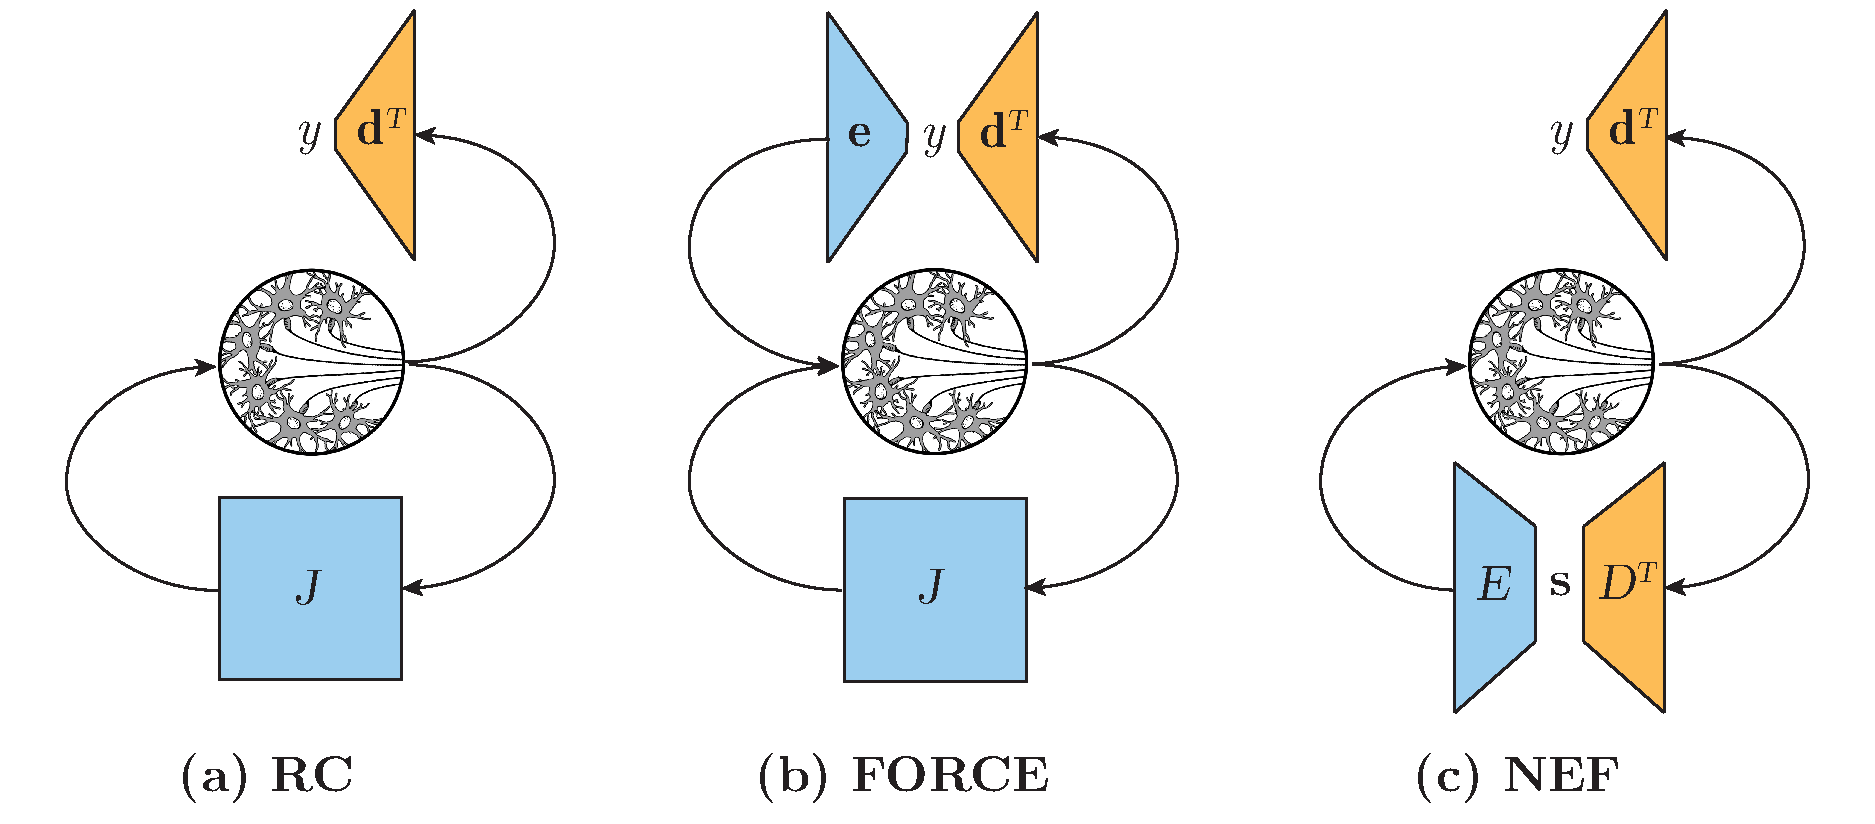
\includegraphics[width=\textwidth]{rc-force-nef}
  \caption{ \label{fig:architectures}
    Comparing the recurrent architectures of (a)~Reservoir Computing~(RC), (b)~First-Order Reduced and Controlled Error~(FORCE), and (c)~the Neural Engineering Framework~(NEF).
    Blue weights are fixed and randomly chosen.
    Orange weights are learned either online or offline.
    Each ensemble is a pool of synapses and neurons that filter and nonlinearly encode the weighted activities.
    The input to each network is omitted for simplicity.
  }
\end{figure}

\TODO{Remove $s$ and replace $J$ with $W$ in figure.}

We now consider the architectural relationships in considerable detail, focusing on the one-dimensional input-output case for notational convenience.
In the case of RC networks (see Figure~\ref{fig:architectures}a), they make a conceptual separation between a fixed {\it reservoir} of randomly-connected neural units, and a learned {\it readout}.
The reservoir is driven by encoding the input signal, $u(t) \in \mathbb{R}$, using a random vector, $\V{e}^\text{in} \in \mathbb{R}^n$.
The units within the reservoir are recurrently connected using a random matrix, $W \in \mathbb{R}^{n \times n}$.
And a feed-forward readout vector, $\V{d} \in \mathbb{R}^{n}$, is optimized to decode some target, $y(t) \in \mathbb{R}$.
%In summary,
%\begin{align} \label{eq:architecture-rc}
%\V{b}(t) &= J \V{a}(t) + \V{e}^\text{in} u(t) \\
%y(t) &= \V{d}^T \V{a}(t) \text{.}
%\end{align}
Intuitively, the reservoir expands the input into a set of nonlinear temporal basis functions---referred to as {\it echoes}---while the readout combines these dynamical traces to approximate the desired target.
Since the readout is typically a linear combination of the reservoir's activity, the decoders may be learned via least-squares regression.
This is equivalent to the optimization performed by the NEF on the output transformation, but using data that is collected by explicitly simulating the network over time.
In contrast, the reservoir is left untrained with dynamical properties that remain fixed, independently of the desired task.

While RC solves the issue of training RNNs, the problem of efficient scaling remains. 
Indeed, as noted by RC theorists, ``just simply creating a reservoir at random is unsatisfactory'' and ``setting up the reservoir such that a good state expansion emerges is an ill-understood challenge in many respects''~\citep{lukovsevicius2012reservoir}.
Generally, the computational power of RC relies upon having a sufficiently large reservoir that represents a high-dimensional superset of the required dynamics, ultimately resulting in an inefficient use of resources for many systems.
This becomes problematic when considering the time and memory required to simulate RC networks, which scales as $\bigoh{ n^2 }$, thus making large-scale simulations of the brain computationally prohibitive.
\TODO{Cite memory limits on random networks.}
In section~\ref{sec:delay-rc} we show that rate-based reservoirs (ESNs) can be outperformed in accuracy, time, and memory, by \emph{spiking} NEF networks of the same size.
%We use the example of a delay line to highlight these limitations.

The First-Order Reduced and Controlled Error~\citep[FORCE;][]{sussillo2009generating} method extends ESNs by learning a low-rank component of the recurrent weight matrix.
This can be decomposed into a separate feedback loop, that \emph{autoencodes} the desired output back into the network (see Figure~\ref{fig:architectures}b).
Specifically, the recurrent weights include an additional outer-product term, $\V{e} \V{d}^T \in \mathbb{R}^{n \times n}$, where $\V{e} \in \mathbb{R}^n$ is a fixed random vector, and $\V{d} \in \mathbb{R}^n$ is the same decoding vector from before.
By design, these weights decode an approximation of the desired output, $y(t)$, and subsequently encode it back into the reservoir, alongside the random mixing from $W$.
This additional loop improves the performance the network, assuming the underlying dynamics are at least partially driven by a static function of the filtered and randomly encoded target signal.
However, this is not always the case.
In section~\ref{sec:force-comparison}, we show that this choice of re-encoding the output signal is sometimes not only suboptimal, but can actually reduce accuracy compared to an equivalent reservoir computer (i.e.,~without the additional FORCE-learned feedback).
The NEF provides a theoretical explanation for why this can sometimes be the case.
These same observations apply to the full-FORCE method~\citep{depasquale2018full}, which learns a full-rank matrix that encodes the same state as in FORCE, but using additional degrees of freedom, similar to \citet{tripp2006neural}.

The Neural Engineering Framework~\citep[NEF;][]{eliasmith1999developing,eliasmith2003a} provides an alternative method for building dynamical neural networks (see Figure~\ref{fig:architectures}c).
Rather than relying on random feedback, or always re-encoding the output (in the case of FORCE), the NEF optimizes the recurrent weights to represent the desired dynamical state.
This can be understood as constructing an RC network with an optimized reservoir, although the approaches were developed independently.
In the NEF, the desired dynamical state, $\V{x}(t) \in \mathbb{R}^q$, is either expressed in closed form as a set of dynamical equations (in continuous-time or discrete-time), or provided via time-series data as is more typical within RC.
Then, the recurrent weight matrix is factored into $ED^T \in \mathbb{R}^{n \times n}$, where $E \in \mathbb{R}^{n \times q}$ is a fixed encoding matrix, $D \in \mathbb{R}^{n \times q}$ is a learned decoding matrix, and a filtered combination of input and recurrent activations represent $\V{x}(t)$.
A central observation made by the NEF is that the optimal $D$ can be determined from $\V{x}(t)$, the selection of neuron models, the models of postsynaptic current~(PSC), and whether the simulation is analog or digital~\citep{voelker2018}.
%\begin{equation}\label{eq:boxed}
%\V{s}(t) = \sum_{i=0}^k c_i \V{x}^{(i)}(t) \text{,} \quad \V{s}[t] = \sum_{i=0}^k \bar{c}_i \V{x}^{[i]}[t] \text{,}
%\end{equation}
%where $c_i$ are the transfer function coefficients of the analog synapse model, or $\bar{c}_i$ for the digital synapse model, respectively~\cite[][equations~17,19]{voelker2017b}.
In the same way as FORCE, the NEF may include $\V{d}$ as a column of $D$, and $\V{e}$ as a column of $E$, to re-encode $y(t)$ -- equivalent to asserting that a filtered version of $y(t)$ is a dimension of $\V{x}(t)$.
This assumption is made if and only if it is helpful~\citep[e.g.,~to perform integration;][]{singh2004}.
If all relevant state-variables are identified, and all target models are ideally leveraged, then the high-dimensional dynamics introduced by $W$ serve absolutely no purpose.
To this point, we find that even the expansion of the input signal into a rich set of nonlinear temporal basis functions can be accomplished by an optimally-designed, closed-form, dynamical system (see section~\ref{sec:nef-delay}).

Now we shift focus to discuss the method(s) of training in some detail (see Table~\ref{tab:learning-types}).
Within the NEF, the important distinction between ESNs and LSMs is captured simply by the choice of $G_i \left[ \cdot \right]$ (see equation~\ref{eq:encoding}).
In either case, we can identify the neural activity of the reservoir with $a_i(t)$, where $\V{x}(t)$ is some \emph{unknown} (latent) state that depends on both $u(t)$ and the dynamical properties of the reservoir.
Note that characterizing $\V{x}(t)$ is precisely the problem faced when trying to understand what information RC networks are representing.
Regardless, the linear readout amounts to the following approximate nonlinear function of $\V{x}(t)$:
\begin{equation} \label{eq:rc}
y(t) \approx \sum_{i=1}^n (a_i \ast h)(t) \V{d}^\V{f}_i \text{.}
\end{equation}
This has the same form as equation~\ref{eq:decoding} from Principle~2 of the NEF.
The important difference lies in how the decoders $D^\V{f}$ are trained.
Rather than solving for $D^\V{f}$ using equation~\ref{eq:decoder_solution}, the network is explicitly simulated to obtain the exact temporal basis functions.
In general, the RC training method relies on \emph{explicit} simulation, since $\V{x}(t)$ is unknown. In the NEF the simulation is typically \emph{implicit} within Principle~2, but can also be made explicit in exactly the same manner~\citep{voelker2016a, duggins2017incorporating}.

\begin{table} 
\centering
  
  \begin{tabular}{@{}lcccccc@{}} \toprule
    & \multicolumn{2}{c}{Recurrence} & \multicolumn{2}{c}{Readout} & \multicolumn{2}{c}{Simulation} \\ 
    \cmidrule(l){2-3} \cmidrule(l){4-5} \cmidrule(l){6-7}
    Method & Online & Offline & Online & Offline & Explicit & Implicit \\ 
    \midrule
    RC & & & & \checkmark & \checkmark & \\
    FORCE & \checkmark & $\thicksim$ & \checkmark & $\thicksim$ & \checkmark & \\
    Full-FORCE & \checkmark & $\thicksim$ & $\thicksim$ & \checkmark & \checkmark & \\
    NEF & $\thicksim$ & \checkmark & $\thicksim$ & \checkmark & $\thicksim$ & \checkmark \\
    \bottomrule
  \end{tabular}
  \caption{ \label{tab:learning-types}
    Summary of the characteristics of each training method. Tildes ($\thicksim$) denote less-commonly advertised, but sensible, use-cases (see text for details).}
%\begin{tabular}{ |c|c|c| } 
%\hline
%  & Online learning & Offline learning \\ 
%\hline
%Explicit simulation & RC* and NEF & RC and NEF  \\ 
%\hline
%Implicit simulation & NEF & NEF \\ 
%\hline
%\end{tabular} \\
\end{table}

The NEF, by default, avoids explicit simulation because it is more costly (especially as the time-step becomes small), which is of practical importance when engineering large-scale networks~\citep[e.g.,][]{eliasmith2012}.
However, the method does have the benefit of automatically refining any additional, non-Gaussian, error in the decoding introduced by the substitution of equation~\ref{eq:rates}.
Furthermore, the readout can learn to compensate for other sources of error and even mischaracterizations of the state-variable.
On the one hand, this can simplify the engineering work involved in training the network, while on the other hand it can mask the effects of costly modelling mistakes.

For the non-adaptive, non-spiking, case the explicit training method adds absolutely no improvement, assuming the representation has been correctly characterized.
Overall, the explicit training methodology is only suitable for black-box applications where there is little-to-no visibility into the latent dynamical state-variables that generated the data, or for when randomized high-dimensional feedback makes it generally intractable to analytically determine the trajectory of the network's dynamics.

From the perspective of RC, the NEF provides a way to solve for the recurrent connection weights by imposing a low-dimensional dynamical state $\V{x}(t)$ on the reservoir.
This can be thought of as building a  \emph{structured} reservoir that is optimized for a restricted subset of functions.
Specifically, we may include a set of temporal basis functions (that incorporate prior knowledge of the desired function) using Principle~3, and then apply any training method to this specially constructed reservoir.
The readout may still capture unanticipated nonlinear relationships between the state and the target, and this readout may still be trained from data.
The NEF provides a way to understand the resulting computations, and to systematically relate the dynamics of the state-variables to the parameters of the computational models.
This allows us to, for instance, understand the network-level effects of including different synapse models.
Furthermore, this reduces the cost of simulation time and memory by a factor of $\bigoh{ n }$ for constant dimensionality, since the number of connection weights for RC scale as $\bigoh{ n^2 }$.

The balanced SNN approach of \citet{boerlin2011spike, boerlin2013predictive} requires a separate discussion.
These methods are closer to the NEF in that they begin with a model of the desired dynamics, and then map that system onto a latent representation within an SNN using factored weight matrices.
These methods do not rely on randomized feedback, nor explicit simulation of the network over time to train its parameters.
Rather, they derive a closed-form solution for the parameters.
These parameters, in effect, deterministically control the spike-timing of each neuron, in such a way that the population collaboratively keeps any deviations from its ideal state bounded above by the peak magnitude of a single filtered and weighted spike, $h(0) \left( \tau n \right)^{-1} = n^{-1}$ (see equation~\ref{eq:lowpass-impulse}).
In particular, each neuron's spike signals a constant deviation from the ideal, which causes all neurons to instantly update their local state to track the global error.
The outcome is precision that scales as $\bigoh{n}$, that is, linearly in the number of neurons, or the total number of spikes~\citep{boahen2017neuromorph}. 
However, this scheme applies only to \emph{linear} dynamical systems, relies on near-instantaneous communication between all neurons with a sufficiently small time-step, and requires linear neurons with relatively minimal leakage and no refractory period~\citep{boerlin2013predictive}.\footnote{
We thank Daniel Rasmussen for having implemented these methods in Nengo~(unpublished),
which served to validate these criticisms and to inform this discussion through additional experimentation.}

The work has been extended to support more biologically-plausible mechanisms, but the scaling becomes $\bigoh{\sqrt{n}}$ as in the NEF~\citep[][Figure~12d]{schwemmer2015constructing}.
In general, it is unclear how far these assumptions can be relaxed before scaling regresses to $\bigoh{\sqrt{n}}$, which is of relevance when considering our targets of modelling biological systems and compiling onto neuromorphic hardware -- both of these targets regularly violate the above assumptions.
As we show, the NEF can account for and remain robust to non-idealities, such as discrete time-steps, higher-order synapses, and detailed neural dynamics.
We find that some of the remaining differences between the statistics of spike-trains, and the number of spikes required to achieve some level of precision, can be made up for in the NEF by delaying spikes a variable length of time that is sensitive to the global error~(unpublished) -- but we cannot currently offer a biologically plausible explanation to learn such a mechanism.
Nevertheless, we believe further investigation into these areas of research are of utmost importance for determining the computationally-theoretic limits of SNN precision with respect to some target set of dynamical primitives, and for maximizing the efficiency of information transmission per spike~\citep[][pp.~92--127]{eliasmith2003a}.

Returning to the literature on RNNs and backpropagation, there exists a range of methods designed to convert a conventionally-trained deep network, that uses static non-spiking (i.e.,~rate-based) nonlinearities, into an equivalent SNN~\citep[][and various methods mentioned in section~\ref{sec:bptt}]{cao2015spiking, rueckauer2017conversion, yousefzadehconversion2019}.
This comes with some minor loss in precision due to spike-variability.
However, these methods on their own do not address the difficulties in training RNNs.
Moreover, they do not immediately extend to recurrent SNNs, that is, unless the RNN has been trained with the same filter as the SNN.
But of equal importance, is that common to all of the methods mentioned above are limitations regarding the nonlinearities employed by both networks.
In particular, they commonly assume rectified linear activation units, corresponding to specifically-engineered integrate-and-fire units in the SNN, which limits the applicability of these methods in the context of biologically-grounded models and implementation on neurormorphic hardware.

\section{Neuromorphic Computing}
\label{sec:neuromorphic}

The term \emph{neuromorphic computing}---also known as neuromorphic engineering---refers broadly to the use of specialized hardware to emulate computational principles of biological nervous systems~\citep{mead1989analog, liu2002analog}.
Here, we focus more specifically on the synthesis of Spiking Neural Networks~(SNNs)---in both analog and digital hardware---for low-power, dynamical, brain-like, computation~\citep{boahen2017neuromorph}.

This section provides a brief overview of the landscape, with an emphasis placed on state-of-the-art hardware made available to the Centre for Theoretical Neuroscience, at the University of Waterloo, for academic research, namely: SpiNNaker~\citep{furber2014spinnaker}, Braindrop~\citep{braindrop2019}, and Loihi~\citep{davies2018loihi}.
At the same time, this overlaps with the efforts of many companies, including: Applied Brain Research~(ABR), Femtosense, Intel, IBM, Numenta, Qualcomm, BrainChip, General Vision, HRL Laboratories, Brain Corporation, Knowm, Samsung, and Vicarious FP~\citep{marketreport2018, femtosense} -- although we focus primarily on ABR's marriage of Nengo and the NEF with neuromorphic hardware from Femtosense (i.e.,~Braindrop) and Intel (i.e.,~Loihi).
A non-exhaustive list of other architectures, many of which implement NEF networks, are provided in section~\ref{sec:neuromorphic-others}.

Coming from a purely computational-theoretic perspective, there is nothing special about neuromorphic hardware; alternative hardware architectures cannot move beyond what is already Turing-computable.
There is no logical nor physical reason to believe that neurons and synapses somehow enable new computations that were previously unable to be emulated using available technology.
Instead, neuromorphic architectures aim to implement specific classes of algorithms, realized via massively-parallelized event-driven computations that are sparse in both space and time, using dramatically less power~\citep{tang2017sparse}.

The human brain has been estimated to consume as little as $10$--$20$\,fJ on average per ``synaptic event''~\citep{cassidy2014real, boahen2017neuromorph}, totalling approximately $20$\,W across its {\textasciitilde{}}\numprint{e11}~neurons and {\textasciitilde{}}\numprint{e14}~synapses~\citep{koch2014}.
After more than $30$ years of work~\citep{cassidy2013design}, the state-of-the-art in neuromorphic computing is on the verge of reaching this level of performance, with Braindrop, Loihi, and TrueNorth~\citep{merolla2014million}, each coming within a factor of \numprint{e1}--\numprint{e3} for roughly equivalent measures of energy per synaptic operation and typical network configurations~\citep{braindrop2019}.
Such potential energy savings are not only tremendous, but a prerequisite to reach the exascale (\numprint{e18}) level of computation achieved by the human brain -- unless one has access to a super-computing cluster powered by a nuclear power plant producing on the order of \numprint{e9}~watts~\citep{furber2012build, neurogrid2014}.
However, such power measurements are not straight-forward to interpret, as there are many other factors such as the cost of scaling, flexibility of the hardware, and open questions surrounding whether the energy per synaptic event is the best metric for evaluating system performance, and how much speed, accuracy, and biological detail is necessary~\citep{eliasmith2013build} -- all of which make fair benchmarking an incredibly challenging problem~\citep{stewart2015closed}.

However, improved power-efficiency often comes with the costs of reduced programmability and narrowed application spaces;
the more you know about the problem that you are trying to solve, the more that can be ``baked in'' to the hardware to save energy and space, while sacrificing flexibility.
This fundamental trade-off between being able to solve fewer problems more efficiently, versus more problems less efficiently, is one that the community as a whole is still trying to navigate.
It appears likely there will be no one-size-fits-all solution, and rather a variety of strategies will be needed to mirror the degrees of architectural specificity observed in the human brain.
Yet, there are many common features between neuromorphic hardware architectures, including: dynamic spike-generation, massive parallelism, memory colocated with computational elements, heterogeneity, sparsity, structured connectivity, minimization of spike traffic and synaptic events, and real-time interfacing.
These features are anticipated to provide robust, scalable, and energy-efficient solutions to the domain of tasks where our brains excel: processing sensory information, language and cognition, and motor behaviours -- all dynamically coupled to the time-scales of our environment.

To fully unlock the potential of such hardware, we require significant advances at the intersection of computer science, computational neuroscience, cognitive modelling, electrical engineering, physics, and mathematics.
This involves discovering new algorithms, developing new frameworks, and training the next generation of programmers to think differently about problems -- but the benefits are far-reaching: real-time computation that can in principle scale up to the perceptual, cognitive, and motor capabilities of the human brain, without requiring the energy production of a nuclear power plant.

In chapter~\ref{chapt:nef-extensions}, we summarize some of the main challenges surrounding the use of neuromorphic hardware, and demonstrate how the NEF solves many of these problems.
More generally, we provide a theoretical framework and extensions to formally understand the class of computations that neuromorphic hardware enables, given its computational elements and constraints, including resource budget and desired precision.
A novel class of algorithms involving temporal computations are explored and analyzed in detail in chapter~\ref{chapt:delays}.
Applications running on neuromorphic hardware are provided in chapter~\ref{chapt:results}.

\subsection{SpiNNaker}

The SpiNNaker\footnote{SpiNNaker stands for ``Spiking Neural Network Architecture''.} project formally began in 2005 as a collaboration between several universities and industrial partners, housed at the University of Manchester, with the primary goals of simulating large-scale SNNs in real-time, and investigating new architectures which ``lead to fundamentally new and advantageous principles for energy-efficient massively-parallel computing''~\citep{spinnakerproject, furber2014spinnaker}.
Secondary goals include providing a balance between power, cost, and programmability, to make SpiNNaker accessible to a wide range of researchers across neuroscience and cognitive modelling communities.

The basic building block of SpiNNaker is a chip multiprocessor~(CMP) containing 18 ARM968 cores and 128\,MB SDRAM~\citep{painkras2013spinnaker, furber2013overview}.
Each core was prescribed to simulate \numprint{e3} spiking neurons and \numprint{e6} synapses, although Nengo's integration doubled this target by achieving \numprint{2000} neurons per core through the use of factorized weight matrices~\citep{mundy2015}.
Each CMP is fully digital, locally synchronous, clocked at some frequency (e.g.,~$200$\,MHz), and allotted some amount of wall time (e.g.,~$1$\,ms) to complete each time-step.
Thus, both neural and synaptic elements are virtualized (i.e.,~reusing the same shared silicon) by time-multiplexing as many computations as possible within each core given the allotted wall time.
Although the limiting factor in scaling each core is predominantly the amount of available SDRAM split between cores, and the volume of spike traffic transmitted between CMPs.
The architecture scales up to $2^{16}$ CMPs---over \numprint{e9}~neurons and \numprint{e12}~synapses---asynchronously connected to one another through a 2D triangular toroidal mesh.
An instantiation that realizes their initial target of 1\% of the human brain, using \numprint{e6} cores, was finally reached as of 2018.

Studies involving power-usage are surprisingly scarce, but one such study demonstrated that scaling to one quarter of a million neurons required less than $30$\,W of power, in the worst-case~\citep{stromatias2013power}, or on the order of \numprint{e5}--\numprint{e6} times more power than a human brain of the same size.\footnote{
The human brain has \numprint{400000} times as many neurons, and uses $20$\,W of power.}
This is a significant improvement upon high-performance computing~(HPC) architectures, which devour at least \numprint{e8} times more power than a human brain~\citep{furber2012build}. 
However, a more recent study by \citet{van2018performance} concluded much more conservatively that SpiNNaker is still a factor of $\numprint{e7}$--$\numprint{e9}$ away from the efficiency of the mammalian brain.\footnote{
The lower-bound on this estimate comes from a hypothetical extrapolation of their results. Furthermore, the range becomes \numprint{e8}--\numprint{e10} if using the estimate of $10$--$20$\,fJ per synaptic event for the brain.}
In this scenario SpiNNaker was outperformed by NEST running on an HPC cluster, and likewise a smaller-scale implementation of an associative memory on SpiNNaker performed comparably to NEST on an Intel Core i7-4710MQ processor~\citep{stockel2017binary}.
Similarly, \citet{knight2018gpus} found that GPUs improved both the simulation time and energy-to-solution for cortical circuit simulations, compared to SpiNNaker and CPU-based HPC hardware.
On the other hand, \citet{sugiarto2016high} estimated that both SpiNNaker and an FPGA provide a $\numprint{e2}$--$\numprint{e3}$-fold improvement over both CPUs and GPUs, on an image processing task. 
Clearly it matters what one is actually scaling towards.

Nengo has been ported to SpiNNaker~\citep{galluppi2012real, mundy2015} and used to run the full Spaun brain model in real-time~\citep{mundy2016real}.
This goal represented a \numprint{e4}-fold speedup over a conventional X86 CPU implementation~\citep{stewart2014large}.
This implementation required significant work by \citet{mundy2016real} to leverage the flexibility of the SpiNNaker architecture, and so we do not go into detail here.
General support has also been added for both supervised learning~\citep{davies2013} and unsupervised learning~\citep{knight2016} to learn human-scale vocabularies online using Nengo (see section~\ref{sec:learn-spinnaker}).
Meanwhile, Nengo has also been deployed on a prototype autonomous robot equipped with a SpiNNaker board to sense and act in real-time~\citep{galluppi2014}.
PyNN has also been ported over to SpiNNaker, further highlighting the flexibility of the architecture~\citep{rhodes2018spynnaker}.
Several other applications of SpiNNaker are reviewed by \citet{rhodes2018spynnaker}, independently of Nengo.

The next generation of SpiNNaker, dubbed SpiNNaker~2, is currently in development with a prototype chip available for testing~\citep{liu2018memory}.
Although Nengo support may not be available any time soon, the hardware promises to improve upon the speed- and power-efficiency of the first generation by use of improved fabrication processes, advanced per-core power management techniques, and specialized hardware acceleration for the exponential function.
\citet{liu2018memory} deploys a deep neural network on the prototype SpiNNaker~2 test chip, realizing power improvements on the order of \numprint{e2} versus a traditional X86 CPU implementation.

\subsection{Braindrop}

Braindrop~\citep{braindrop2019} is a mixed-signal---both analog and digital---neuromorphic architecture that attempts to realize the energy-efficiency of the human brain, without sacrificing the flexibility required to simulate functional large-scale cognitive systems such as Spaun~\citep{eliasmith2012}.
This project was a five year collaboration between Stanford, Yale, and the University of Waterloo, and was made possible in this time frame 
by building upon many of the tools and lessons learned from its predecessor, Neurogrid~\citep{neurogrid2014}. 

Both Neurogrid and Braindrop take a dynamical systems-based approach~\citep{arthur2011silicon, gao2012dynamical} to realize network-level computation.
In particular, the device-level physics of subthreshold analog circuits~\citep{andreou1991current}---emulating the behaviours of neurons and synapses---are leveraged by weighting the digital communication of spikes, to engineer dynamical systems~\citep{dethier2011brain}.
It is argued that an appropriate mixture of analog computation for nonlinear encoding---sparsifying signals across both space and time---and digital communication for spike transmission, is responsible for the energy-efficiency of mamillian brains~\citep{boahen2017neuromorph}.
This hypothesis makes such architectures a natural target for NEF networks, in particular due to its modelling of the dynamical primitives encoding signals into spikes, and its efficient procedures to solve for the weights in the communication fabric.

The NEF has been deployed on Neurogrid primarily to implement control algorithms~\citep{dethier2011brain, choudhary2012silicon, menon2014controlling}.
However, the use of Neurogrid requires advanced calibration~\citep{kauderer2017calibrating} and temperature-compensation techniques~\citep{abrams2017} in order to tame the analog variability -- both of which contribute to it being difficult to use in practical applications.\footnote{
For example, a live demonstration that used Neurogrid to control a robotic arm, which had previously worked within an air-controlled climate, no longer functioned in the conference hall as it was bombarded by the warmth of onlookers~[personal communication].}

Braindrop is designed explicitly with Nengo and the NEF in mind, by way of a novel mapping~\citep{voelker2017iscas, neckar2018optimizing}, accompanied by a number of inventive solutions including: temperature-invariance~\citep{abrams2017, reidpint2019, benjamintemp2019}, H-tree routing~\citep{fokserial2018}, sparse encoding by spatial convolution~\citep{feinstein1988hexagonal, braindrop2019}, and decoding by accumulative spike-thinning~\citep{fokthinning2019}.
Of key notability is the fact that Braindrop, in essence, implements a factorization of the weight matrices akin to equation~\ref{eq:factored-weights}, which has cut down on area requirements for SRAM and permitted the sharing of synaptic circuitry across neurons, in turn leading to an estimate of 381~fJ\footnote{
One femtojoule~(fJ) is equivalent to \numprint{e-15} joules~(J).}
per equivalent synaptic operation for network configurations typical in Spaun.
A significant amount of detail addressing the design of the chip is available in \citet{neckar2018braindrop, fok2018communicating, braindrop2019}.
The success of this project has prompted the formation of a start-up company, Femtosense, named after the mere femtojoules that synapses consume to sense and react~\citep{femtosense}. 

As stated above, the design of Braindrop is informed by many of the lessons learned from Neurogrid.
Detailed models have been studied at the circuit level~\citep{benjamintemp2019} and NEF-related methods have been employed at the network level~\citep{voelker2017iscas, reidpint2019}, in order to simultaneously tame and account for the non-idealities introduced by transistor mismatch, parasitic capacitances, and temperature variation.
In chapter~\ref{chapt:nef-extensions}, we expose a few of these extensions at a theoretical level.
In chapter~\ref{chapt:results}, we provide applications that demonstrate robust dynamical computation on Braindrop.

\TODO{Mention some details about how the NEF is realized, or point forward to the methods section and say stuff there, while acknowledging Terry again and not taking credit myself.}

% Multicast tree router \citep{merolla2014multicast}

\subsection{Loihi}

Loihi~\citep{davies2018loihi} is Intel's fully digital, barrier-synchronized, clock-driven neuromorphic architecture, that promotes significant flexibility in its SNN feature set, while being optimized for low power consumption.
It consists of 128 ``neuromorphic cores'' that operate asynchronously from one another.
Each core time-multiplexes \numprint{1024} neural units---configurable as trees of neurons and dendritic compartments---across the same shared silicon.
In contrast to SpiNNaker, barrier messages are transmitted between cores in order to keep the system synchronized to a global time-step.
This has the advantages of each step only taking as long as it needs\footnote{
One algorithmic time-step may take longer than the next, if for example learning rules are applied irregularly, or depending on the total volume of spike-traffic.} 
while guaranteeing globally deterministic behaviour.

By virtue of being fully digital and barrier-synchronized, there exists far fewer challenges presented to its users when compared to solutions in the mixed-signal, purely analog, or asynchronous digital domains; in particular, the behaviour of the chip is guaranteed to be reliable and predictable.
When compared to simulating SNNs on traditional hardware (e.g.,~an x86~CPU), the challenges that remain include quantization (i.e.,~truncation) of real values (e.g.,~weights, synaptic states, and neuronal states) due to the limited bit-precision of floating-point numbers (1--9~bits), and constraints on connectivity, memory, and bandwidth.
A Loihi emulator, provided by Applied Brain Research~(ABR), accurately reproduces many of these limitations using detailed software models of the underlying hardware~\citep{blouw2018a}.
In addition, software tools exist to map SNNs onto Loihi while optimizing for power-efficiency with respect to the constraints imposed by the hardware~\citep{lin2018programming, lin2018mapping}.

Loihi supports a broad variety of features that make it accessible to a wide range of researchers experimenting with the synthesis of large-scale SNNs.
For example, stochastic noise can be added to internal states, discrete delays may be introduced to spikes and PSCs, synapses can have higher-order dynamics, dendritic trees may be constructed by repurposing the neural units within each core, neuron models may include adaptive terms, learning rules are described using a general template, and finally there is support for several weight compression formats, spike multicast, and closed-loop control via embedded x86 cores~\citep{davies2018loihi}.

ABR has ported Nengo over to Loihi and used the NEF to simulate a nonlinear adaptive controller on a robotic arm~\citep[][and personal communication]{dewolf2016}.
However, Loihi does not support the use of factored weight matrices, meaning that a substantial benefit of the NEF---namely, a linear reduction in the number of multiplies and memory accesses per time-step---is not leveraged at the hardware level.
As a way to resolve this at the software level, Nengo currently creates intermediate populations to represent latent variables explicitly in spikes, which has the adverse effects of amplifying representational error, increasing the number of neurons, and introducing additional rounds of filtering between layers.
Alternatively, weight matrices can be left unfactored and fully-connected, but this misses out on potentially dramatic savings.
\TODO{Cite nengo-loihi github and forward reference methodology section with more details (similar to braindrop).}

Nengo~DL~\citep{rasmussen2018nengodl} has been used to implement a fully-connected deep network performing keyword spotting, on Loihi, while outperforming state-of-the-art hardware in energy cost per inference~\citep{blouw2018a}.
After extensive review of the literature, we have found this to be the first, and currently only published example, outside of Intel's demonstration of sparse pattern representation~\citep{tang2017sparse, davies2018loihi}, to deploy an SNN on the actual chip.

However the flexibility and digital nature of Loihi comes at the cost of increased power-consumption relative to fully analog or mixed-signal architectures. 
Simulations from \citet{davies2018loihi}, that are summarized in \citet[][Table~3]{braindrop2019}, indicate that Loihi consumes on the order of \numprint{24}~pJ\footnote{
One picojoule~(pJ) is equivalent to \numprint{e-12}~J, or \numprint{e3}~fJ.}
per synaptic operation -- or two orders-of-magnitude more than Braindrop's equivalent measure.
Regardless, the analog variability intrinsic to Braindrop changes the scope of target applications, and moreover the results of Loihi still demonstrate a three orders-of-magnitude improvement over a comparable solution running on a CPU.
We speculate the power-efficiency of Loihi can be improved somewhat by supporting factored weight matrices, and refining the architecture according to the network topology and particular features leveraged by the example application.

On the other hand, it is currently unclear how important or useful each of Loihi's features are relative to one another, and especially in the context of target applications.
We believe that an important avenue of research, and the role of Nengo and the NEF in this context, is to facilitate such exploration, by systematically harnessing relevant features for useful computation, which can then feed back to co-design future iterations (as was the case for Neurogrid and Braindrop).
More generally, specific classes of computations that leverage particular subsets of features will encounter distinct trade-offs when it comes to resource usage, precision, energy-to-solution, and time-to-solution; mathematical frameworks, such as the NEF, participate by providing a unified way of characterizing such trade-offs.
A primary focus of chapters~\ref{chapt:nef-extensions}--\ref{chapt:results} is to take a concrete step in these directions by explicitly incorporating some of Loihi's features into the NEF and demonstrating dynamical systems functioning on the physical hardware.

\subsection{Others}
\label{sec:neuromorphic-others}

The literature on neuromorphic computing is incredibly extensive\footnote{%
See \citet{schuman2017survey} for a review that references nearly \numprint{3000} other papers.}%
, dating back to the late 80's and recently displaying a renewed set of interests spanning many historically-separate communities.
This has resulted in a number of architectures mentioned below, which were not made available to us, to be considered outside the scope of this thesis.
A number of excellent review articles by experts widely regarded to have advanced the field, are made available by \citet{bartolozzi1999neuromorphic}, \citet{indiveri2011neuromorphic}, \citet{cassidy2013design}, \citet{cummings2018}, and \citet{rajendran2019low}.
At a higher level, a review that considers the role of biomimicry---the emulation of nature's solutions in order to solve real-world problems---in the context of power-efficient SNNs and neuromorphic computing, is provided by \citet{krichmar2018making}.

Some of the earliest examples of neuromorphic engineering date back to the work of \citet{sivilotti1985novel, mead1988silicon, boahen1989heteroassociative, mahowald1991silicon}.
Many of these techniques have since been extended and scaled up to show-case a large variety of analog, digital, and mixed-signal systems (excluding those mentioned thus far):
Spikey~\citep{pfeil2013six},
BrainScaleS~\citep{schemmel2010wafer, aamir2018mixed, aamir2018accelerated},
DYNAPs~\citep{moradi2018scalable},
IBM's TrueNorth~\citep{merolla2011digital, merolla2014million, esser2016convolutional},
Sydney's DeepSouth~\citep{cummings2018},
ODIN~\citep{frenkel2018},
ROLLS~\citep{qiao2015reconfigurable, glatz2018adaptive},
COLAMN~\citep{wijekoon2012vlsi},
STPU~\citep{smith2017novel},
DANNA~\citep{daffron2016extensions, mitchell2018danna},
and many other related prototypes~\citep[e.g.,][]{glackin2009hardware, moradi2011vlsi, brink2013computing, moradi2014event, park201465k, azghadi2015programmable, binas2016precise, kim2018efficient, chen20184096, zheng2018low, larras2018fully}.

\TODO{Analog computing in a modern context: A linear algebra accelerator case study?}
% A digital neurosynaptic core using embedded crossbar memory with 45 pJ per spike in 45 nm, (GoldenGate SyNAPSE IBM)
\TODO{Missing ASIC results for deep learning?}

Among these systems, a number support the compilation of NEF networks, including a VLSI prototype~\citep{corradi2014}, several FPGA implementations~\citep{naylor2013managing, wang2014compact, berzish2016, wang2017neuromorphic} including ABR's own FPGA backend~(unpublished), several GPUs~\citep{bekolay2014, rasmussen2018nengodl, blouw2018a}, and most recently, TrueNorth~\citep{fischl2018}.

An emerging framework called the Neural and Synaptic Array Transceiver~\citep[NSAT;][]{detorakis2018neural}, which focuses on data-driven autonomy via online learning on neuromorphic hardware, has been validated on a field-programmable gate array~(FPGA).
Likewise, an engine that repurposes generic computational elements in order to flexibly support a variety of network topologies at scale, has been used to implement polychronous SNNs on an FPGA~\citep{wang2013neuromorphic, wang2018breaking}.

There also exist multiple proposals to leverage memristors as an alternative hardware primitive for SNN computation in mixed-signal neuromorphic architectures, due to their compact and non-volatile (i.e.,~maintains memory without power) properties~\citep{payvand2018neuromorphic}.
Several investigations are currently underway to explore the practical challenges associated with these proposals~\citep[e.g.,][]{chang2013building, kudithipudi2016design, cady2018full, boybat2018neuromorphic}.

Likewise, many other unconventional substrates for SNNs are actively being explored, such as nanoscale spintronic oscillators and multiferroic devices~\citep{torrejon2017neuromorphic, hoppensteadt2017applied, manipatruni2018beyond}, analog non-volatile memory~\citep{ambrogio2018equivalent}, organic electronics~\citep{van2018organic}, phase-change oxides~\citep{zhao2019low}, photonics~\citep{tait2018silicon, shainline2018largest}, and superconducting circuits based on quantum phase-slip junctions~\citep[QPSJs;][]{cheng2019superconducting}.

